\documentclass{book}

\usepackage{../Package/latexa}
\usepackage{../Package/algebra}
\usepackage{../Package/theorema}
\usepackage{../Package/diagramma}
\usepackage{../Package/categoria}

\usepackage{tikz}
\usepackage{tikz-cd}
\usetikzlibrary{arrows}

\newcommand{\qi}{\backsimeq_{\textsc{QI}}}
\newcommand{\ba}{\backsimeq_{\textsc{BA}}}
\newcommand{\normal}{\vartriangleleft}
\newcommand{\tm}{\subset}
\newcommand{\Stab}[2]{\textsf{Stab}_{#1}(#2)}
\newcommand{\Cay}[2]{\textsf{Cay}(#1,#2)}


\renewcommand{\A}{\mathbb{A}}
\newcommand{\Nc}{\mathcal{N}}


\renewcommand{\d}{\textsf{d}}
\renewcommand{\P}{\mathbb{P}}

\newcommand{\af}{\mathfrak{a}}
\newcommand{\Af}{\mathfrak{A}}
\renewcommand{\bf}{\mathfrak{b}}
\newcommand{\Bf}{\mathfrak{B}}
\newcommand{\cf}{\mathfrak{c}}
\newcommand{\Cf}{\mathfrak{C}}
\newcommand{\ff}{\mathfrak{f}}
\newcommand{\Ff}{\mathfrak{F}}
\newcommand{\pf}{\mathfrak{p}}
\newcommand{\Pf}{\mathfrak{P}}
\newcommand{\mf}{\mathfrak{m}}
\newcommand{\Mf}{\mathfrak{M}}
\newcommand{\qf}{\mathfrak{q}}
\newcommand{\Qf}{\mathfrak{Q}}

\renewcommand{\M}{\mathbb{M}}
\renewcommand{\l}[1]{\overline{#1}}

\newcommand{\Ac}{\mathcal{A}}
\newcommand{\Rc}{\mathcal{R}}
\renewcommand{\O}{\mathcal{O}}

\newcommand{\Frob}{\textsf{Frob}}

\newcommand{\Leg}[2]{\left(\frac{#1}{#2}\right)}

\newcommand{\ric}{\textsf{ric}}
\newcommand{\g}{\mathfrak{g}}
\newcommand{\kf}{\mathfrak{k}}
\newcommand{\p}{\mathfrak{p}}
\newcommand{\m}{\mathfrak{m}}

\newcommand{\GL}{\textsf{GL}(n,\R)}
\newcommand{\glf}{\mathfrak{gl}(n,\R)}
\newcommand{\SO}{\textsf{SO}(n,\R)}
\newcommand{\so}{\mathfrak{so}(n,\R)}
\newcommand{\SL}{\textsf{SL}(n,\R)}
\newcommand{\slf}{\mathfrak{sl}(n,\R)}
\newcommand{\POS}{\textsf{Pos}(n,\R)}
\newcommand{\symm}{\textsf{symm}(n,\R)}
\newcommand{\of}{\mathfrak{o}}

\usepackage{enumerate}

\makeindex

\begin{document}

\title{
\begin{huge}
Differentialgeometrie 2\\
\end{huge}
\begin{large}
Kurzskript, WS 16/17
\end{large}}


\author{Ak\i n Ünal}
\maketitle
\renewcommand{\i}{^{-1}}

Das folgende Kurzskript orientiert sich an einer Vorlesung, die im Wintersemester 2016 / 2017 in Heidelberg gehalten wurde. Für alle Fehler im Text trägt ausschließlich der Autor die Verantwortung.

\setcounter{tocdepth}{1}
\tableofcontents


\chapter{Erste Woche}
\section{Krümmungen}

\Def{}
Es sei $M$ eine Riemannsche Mannigfaltigkeit und $\kappa_p(\sigma)$ bezeichne die Schnittkrümmung in einem Punkt $p$ und einer Ebene $\sigma \subset T_pM$.\\
$M$ heißt \df{von positiver Schnittkrümmung}, falls $\kappa_p(\sigma) > 0$ für alle $p \in M, \sigma \subset T_pM$.\\
Bezeichnet $\ric$ die Ricci-Krümung, so heißt $M$ \df{von positiver Ricci-Krümmung}, falls $\ric_p(v,v) > 0$ für alle $p \in M, v \in T_pM$.\\
Die Ricci-Krümmung von $M$ wird von $\alpha > 0$ \df{nach unten beschränkt}, falls
\[ \ric_p(v,v) \geq \alpha g_p(v,v) \]
für alle $p \in M, v \in T_pM$.

\Def{Isometrien}
Eine glatte Abbildung $f : M \pfeil{} N$ heißt \df{lokal isometrisch}, falls für alle $p \in M$ das Differential $\d f_p : T_pM \pfeil{} T_pN$ eine lineare Isometrie metrischer Räume ist.

\Bem{}
$f$ ist genau dann isometrisch, wenn $f$ lokal isometrisch und diffeomorph ist.

\Satz{}
Jede glatte Abbildung $f : M \pfeil{} M$, die für einen Punkt eine Isometrie auf den Tangentialräumen induziert, ist eine Isometrie.\\
Jede glatte, abstandserhaltende Funktion $f : M \pfeil{} M$ ist eine Isometrie.

\Def{}
Die \df{Kompakt-Offen-Topologie} auf $\textsf{Isom}(M,M)$ wird durch eine Basis folgender Mengen generiert
\[ W(K,U) := \set{f}{ f(K) \subseteq U } \]
für alle $K \subseteq M$ kompakt und $ U \subseteq M$ offen.

\Prop{Cartan}
Seien $v,w$ normierte, orthogonale Vektoren in $T_pM$. Es gilt
\[ d(c_v(t), c_w(t))^2 = 2t^2 - \frac{\kappa_p(\sigma_{v,w})}{6} t^4 + o(t^5)  \]

\Lem{}
Ist $J$ ein Jacobifeld entlang $c$, so gilt
\[ D_t(\Rc (\dot{c}, J), \dot{c})(0) = \Rc (\dot{c}, D_tJ)\dot{c}  \]
\begin{Beweis}{}
\begin{align*}
\frac{\d}{\d t} g(\Rc(\dot{c} , J) \dot{c}, w ) &= g(D_t \Rc(\dot{c}, J) \dot{c}, w ) + g(\Rc (\dot{c}, J) \dot{c}, D_tw )\\
\frac{\d}{\d t} g(\Rc(\dot{c} , w) \dot{c}, J ) &= g(D_t \Rc(\dot{c}, w) \dot{c}, J ) + g(\Rc (\dot{c}, w) \dot{c}, D_tJ )\\
g(D_t \Rc(\dot{c}, J) \dot{c}, w ) &= g(D_t \Rc(\dot{c}, w) \dot{c}, J ) + g(\Rc(\dot{c}, w) \dot{c}, D_tJ ) =  g(\Rc(\dot{c}, D_tJ) \dot{c}, w )
\end{align*}
\end{Beweis}


\Prop{}
Seien $v,w \in T_pM$ mit $\bet{w} = 1$. Setze $J(t) = (\d \exp_p)_{tv}(tw) \in \J_{c_v}$. Dann gilt
\[ \bet{J(t)}^2 = g(J(t), J(t)) = t^2 - \frac{1}{3} g(\Rc(v,w)w, v)t^4 + o(t^5) \]

\begin{Beweis}{}
Es gilt
\[ J(0) = 0 \text{ und } D_t(J)(0) = w \]
Man rechnet nach
\begin{align*}
	g(J,J)(0)     & = 0                                                                    \\
	g(J,J)'(0)    & = \frac{\d}{\d t}_{|t = 0} g(J(t), J(t)) = 2g(D_t(J),J) (0) = 0        \\
	g(J,J)''(0)   & = 2g(D_tJ, D_tJ)(0) + 2g(D_tD_tJ,J)(0) = 2g(w,w) = 2                   \\
	g(J,J)'''(0)  & = 6g(D_tD_tJ, D_tJ)(0) = 6g(-\Rc(\dot{c}, J) \dot{c}, D_t J ) (0) = 0  \\
	g(J,J)''''(0) & = 8g(\Rc(\dot{c}, D_tJ )\dot{c}, D_tJ  ) - \frac{8}{24} g(\Rc(v,w)w,v) = - \frac{1}{3}g(\Rc(v,w)w,v)
\end{align*}
\end{Beweis}

\newpage
\chapter{Erster Teil, Räume Konstanter Krümmung}
\section{Zweiter Fundamentaltensor}
\Def{}
Unter $\M_\kappa^n$ verstehen wir die bis auf Isometrie eindeutige vollständige, einfache zusammenhängende, $n$-dimensionale Riemannsche Mannigfaltigkeit von konstanter Schnittkrümmung $\kappa$.
\Bem{}
Skaliert man die Metrik einer Riemannschen Mannigfaltigkeit mt $c > 0$, so skaliert sich ihre Krümmung mit $\frac{1}{c}$.
\Bsp{}
Man führe auf $\R^{n+1}$ folgende Bilinearformen ein
\begin{align*}
(x,y) &:= \sum_{i = 1}^{n+1}x_i \cdot y_i\\
\shrp{x,y} &:= \sum_{i = 1}^{n}x_i \cdot y_i - x_{n+1} \cdot y_{n+1}\\
\end{align*}
Dann gilt
\begin{align*}
\M_0^n = \R^n && \M_1^n = S^n = \{x \in \R^{n+1} ~|~ (x,x) = 1\} && \M_{-1}^n = \H^n = \{ x \in \R^{n+1} ~|~ \shrp{x,x} = -1, x_{n+1} > 0 \} 
\end{align*}

\Def{}
Der \df{Index} einer symmetrischen Bilinearform ist die größte Dimension aller Unterräume, auf denen jene Bilinearform negativ definit ist.

\Def{}
Sei $(M,g)$ eine semi-Riemannsche Untermannigfaltigkeit einer semi-Riemannschen Mannigfaltigkeit $(\l M,\l g)$. Bezeichnet $\iota : M \inj{} \l M$ die Einbettung, so verstehen wir unter $\l\V(M) := \Gamma(\iota^*(\T\l M))$ den Pullback der Vektorfelder auf $\l M$, d.h.
\[ \l\V(M) = \set{Y_{|M}}{Y \in \V(\l M)} \]
Unter $\V(M)^\bot \subset \l \V(M)$ verstehen wir die Vektorfelder auf $M$, die normal zu $M$ liegen.\\
Wir schränken den Levi-Civita-Zusammenhang von $\l M$ auf $\V(M) \times \l\V(M)$ ein und erhalten
\[ \l\D : \V(M) \times \l\V(M) \Pfeil{} \l\V(M) \]
Betrachte folgende Zerlegung
\[ T_p\l M = T_pM \oplus (T_pM)^\bot \]
Unter dem \df{Koindex von $M$} verstehen wir den Index auf $(T_pM)^\bot$. Es gilt
\[ \text{Index}(T_p\l M) = \text{Index}(T_pM) + \text{Index}(T_pM)^\bot \]

\Lem{}
$\l\D$ ist wohldefiniert.
\begin{Beweis}{}
Sei $p \in M$ ein Punkt und $U \subset M$ eine Koordinatennachbarschaft von $p$. Seien ferner $V \in \V(M), X \in \l\V(M)$ mit Liftungen $\l{V},\l{X} \in \V(\l M)$. $\l{X}$ lässt sich auf $U$ darstellen durch
\[ \l{X} = \sum_{i} f_i \frac{\d}{\d x_i} \]
\[ \l\D_{\l{V}}\l{X} = \sum_i \l{V}(f_i) \frac{\d}{\d x_i} + \sum_i f_i \l\D_{\l{V}}\klam{\frac{\d}{\d x_i}} \]
Für $q \in U\cap M$ gilt
\[\l{V}(f_i)(q) = V_q(f_i) = V_q((f_i)_{|U\cap M}) \]
und
\[ \l\D_{\l{V}}\klam{\frac{\d}{\d x_i}}(q) = \l\D_{\l{V}_q}\klam{\frac{\d}{\d x_i}} \]
\end{Beweis}
\Kor{}
Seien $V,W \in \V(M), X,Y \in \l \V(M)$.
\begin{itemize}
\item $\l \D_VX$ ist $\F(M)$-linear in $V$.
\item $\l\D_VX$ ist $\R$-linear in $X$.
\item $\l\D_V(fX) = (Vf) X + f\l\D_VX$
\item $[V,W] = \l\D_VW - \l\D_WV$
\item $Vg(X,Y) = g(\l \D_VX, Y) + g(X, \l \D_VY)$
\end{itemize}
\Lem{}
Sind $V,W \in \V(M)$, dann gilt
\[ \D_VW = (\l\D_VW)^T \]
\begin{Beweis}{}
Sei $X \in \V(M)$ beliebig
\begin{align*}
2g(\l{\D}_{\l{V}}\l{W}, \l{X}) = \l{V}g(\l{W},\l{X}) + \l{W}g(\l{X},\l{V}) - \l{X}g(\l{V},\l{W}) + g(\l{W},[\l{X},\l{V}]) + g(\l X, [\l V,\l W])
\end{align*}
Mit dem Vorhergehenden Korollar erhalten wir durch Einschränkung auf $M$
\[ g(\l{\D}_{V}W, X) = g(\D_{V}W, X) \]
Es gilt ferner
\[ g(\l{\D}_{V}W, X) = g((\l{\D}_{V}W)^T, X) \]
da $X$ tangential an $M$ liegt.
\end{Beweis}

\Lem{}
Definiere den \df{Gestalttensor} bzw. \df{zweiten Fundamentaltensor} durch
\begin{align*}
\Pi : \V(M) \times \V(M) &\Pfeil{} \V(M)^\bot\\
(V,W) & \longmapsto (\l\D_VW)^N = \l\D_VW - \D_VW
\end{align*}
Dann ist dieser Tensor $\F(M)$-bilinear und symmetrisch.
\begin{Beweis}{}
\begin{align*}
(\l\D_V(fW))^N = (f\l\D_VW)^N + (V(f) W)^N = (f\l\D_VW)^N\\
\Pi(V,W) - \Pi(W,V) = (\l\D(V,W) - \l\D(W,V))^N = [V,W]^N = 0
\end{align*}
\end{Beweis}

\Satz{Gauss-Gleichung}
Seien $V,W,X,Y \in \V(M)$. Es gilt
\[ g(\Rc(V,W)X,Y) = g(\l{\Rc}(V,W)X,Y) + g(\Pi(V,X), \Pi(W,Y )) - g(\Pi(V,Y), \Pi(W,X )) \]
\begin{Beweis}{}
\begin{align*}
\Rc(X,Y)Z &= -\D_{[X,Y]}Z + [\D_X,\D_Y]Z\\
g(\l{\D}_{[V,W]}X,Y) &= g(\D_{[V,W]}X,Y)\\
g(\l{\D}_V\l{\D}_WX,Y) &= g(\l{\D}_V\D_WX,Y) + g(\l{\D}_V \Pi(W,X), Y)\\
&= g(\D_V\D_WX,Y) + (Vg(\Pi(W,X), Y) - g(\Pi(W,X), \l{\D}_VY ))\\
\end{align*}
Nun gilt aber
\[ g(\Pi(W,X), Y) = 0 \]
Ergo
\begin{align*}
g(\l{\D}_V\l{\D}_WX,Y) &= g(\D_V\D_WX,Y) + (Vg(\Pi(W,X), Y) - g(\Pi(W,X), \l{\D}_VY ))\\
&= g(\D_V\D_WX,Y) -g(\Pi(W,X), \Pi(V,Y) )
\end{align*}
\end{Beweis}

\Kor{}
Sind $v,w \in T_pM$ linear unabhängig, so gilt
\[ \kappa(v,w) = \l{\kappa}(v,w) + \frac{g(\Pi(v,v), \Pi(w,w)) - g(\Pi(v,w), \Pi(v,w))}{g(v,v) g(w,w) - g(v,w)^2} \]

\Prop{}
Sei $Y$ ein Vektorfeld tangential zu $M$ entlang einer Kurve $\alpha(t)$ in $M$. Dann gilt
\[ \l\D_t Y = \D_tY + \Pi(\dot{\alpha}, Y) \]

\Kor{}
$\alpha$ ist genau dann eine Geodäte von $M$, wenn $\l{\D}_t(\dot{\alpha})$ normal zu $M$ steht.

\Def{}
Eine \df{semi-Riemannsche Hyperfläche} ist eine \df{semi-Riemannsche Untermannigfaltigkeit} der Kodimension Eins.

\Def{}
Das \df{Vorzeichen} einer semi-Riemannschen Hyperfläche $M$ ist definiert durch
\[ \e := \left\lbrace 
\begin{aligned}
+1 && \textsf{coindex}M = 0\\
-1 && \textsf{coindex}M = 1
\end{aligned}
\right. \]

\Def{}
Sei $U$ ein normiertes Normalenvektorfeld einer semi-Riemannschen Hyperfläche $M$. Dann wird durch
\[ g(S(V),W)  = g(\Pi(V,W), U)\]
ein (1,1)-Tensorfeld $S$ auf $M$ definiert, der sogenannte \df{Gestaltoperator}, der durch $U$ induziert wird.

\Lem{}
Für alle $v \in T_pM$ gilt
\[ S(v) = -\l{\D}_vU \]
Ferner ist $S_p$ selbstadjungiert.
\begin{Beweis}{}
$g(U,U)$ ist konstant gleich 1. Ergo gilt
\[ g(\l{\D}_VU,U) = 0 \]
Daraus folgt, dass $\l{\D}_VU$ für alle $V \in \V(M)$ tangent an $M$ liegt.\\
Sei nun $W \in \V(M)$, dann gilt
\[ g(S(V),W) = g(\Pi(V,W), U) =g(\l{\D}_VW, U) \gl{g(U,W) = 0} g(\l{\D}_VU,W)   \]
\end{Beweis}

\Kor{}
\[ \kappa(v,w) = \l{\kappa}(v,w) + \e \frac{g(Sv,v)g(Sw,w) - g(Sv,w)^2}{g(v,v) g(w,w) - g(v,w)^2} \]
\begin{Beweis}{}
\[ \Pi(v,w) = \e g(Sv,w) U \text{ und } g(U,U) = \e \]
\end{Beweis}

% % % Vorlesung
\newpage
\section{Hyperbolische Modelle}
\Def{3 Shades of Artig-Sein}
Sei $x \in \R^{n+1}$
\begin{align*}
x \text{ heißt } \left\lbrace \begin{aligned}
\text{\df{zeitartig}, falls } &\shrp{x,x} < 0\\
\text{\df{lichtartig}, falls } &\shrp{x,x} = 0\\
\text{\df{raumartig}, falls } &\shrp{x,x} > 0
\end{aligned} \right.
\end{align*}

\Prop{}
Sei $M = \set{p \in \R^{n+1}}{\shrp{p,p} = -r^2}$. Dann ist $M$ eine Riemannsche Mannigfaltigkeit der konstanten Schnittkrümmung $-\frac{1}{r^2}$ für $r > 0$.
\begin{Beweis}{}
Definiere $f : \R^{n+1} \pfeil{} \R$ durch $x \mapsto \shrp{x,x}$. Dann ist $\d f_p(v) = 2\shrp{v,p}$. Ergo ist $\d f_p$ surjektiv für alle $p \in M$. Ergo ist $f\i(-r^2)$ eine glatte Hyperfläche von $\R^{n+1}$.\\
Ferner ist
\[ T_pM = \Ker \d f_p  = \set{v \in \R^{n+1}}{\shrp{p,v} = 0} = p^\bot \]
Da $p$ zeitartig ist, ist $T_pM$ positiv definit. Ferner ist der vom Einheiten-Normalen Vektorfeld $U(p) = \frac{p}{r}$ abgeleitete Gestaltoperator gegeben durch $S(V) = - \D'_VU = \frac{-V}{r}$. Es folgt
\[ \kappa(v,w) = 0 - \frac{1}{r^2} = - \frac{1}{r^2} \] 
\end{Beweis}

\Def{}
Unter einer \df{Paar-Isometrie} $\Phi : (M,M') \pfeil{} (N,N')$, wobei $M \subset M', N \subset N'$ semi-Riemannsche Mannigfaltigkeiten sind, ist eine Isometrie $M' \pfeil{} N'$, dergestalt, dass auch ihre Restriktion $M \pfeil{} N$ eine Isometrie ist.

\Lem{}
Eine Paar-Isometrie $\Phi : (M,M') \pfeil{} (N,N')$ erhält den Gestalttensor, d.\,h.
\[ \d \Phi (\Pi (v,w)) = \Pi ( \d \Phi(v),\d \Phi(w) ) \]
für alle $p \in M, v,w \in T_pM$.

\Prop{}
Seien $p,q \in M = \set{p \in \R^{n+1}}{\shrp{p,p} = -r^2}$ mit ONBs $e_i \in T_pM, f_i \in T_qM$. Dann existiert eine eindeutige Paar-Isometrie
\[ \phi : (\R^{n+1}, M) \Pfeil{} (\R^{n+1}, M) \]
mit
\begin{align*}
\phi(p) = q \text{ und } \d \phi_p(e_i) = f_i
\end{align*}


\Def{}
Eine semi-Riemannsche Untermannigfaltigkeit $M \subset M'$ heißt \df{total geodätisch}, falls $\Pi = 0$.

\Prop{}
Für eine semi-Riemannsche Untermannigfaltigkeit $M \subset M'$ sind folgende Aussagen äquivalent:
\begin{enumerate}[1.)]
\item $M$ ist total geodätisch in $M'$
\item Jede Geodäte von $M$ bleibt eine Geodäte in $M'$
\item Für $v \in T_pM \subset T_pM'$ liegt das Anfangstück von $\gamma(t) = \exp'_p(tv)$ in $M$. ($\exp'$ bezeichnet hier die Exponentialfunktion von $M'$.)
\item Für jeden Weg in $M$ stimmt der Paralleltransport in $M$ mit dem in $M'$ überein.
\end{enumerate}

\Prop{}
Seien $M, N \subset M'$ vollständige, zusammenhängende, total geodätische semi-Riemannsche Mannigfaltigkeiten. Existiert ein Punkt $p \in M\cap N$ mit
\[ T_pM = T_pN \] 
so folgt
\[ M = N\]

\Prop{}
Bezeichnet $H^n \subset \R^{n+1}$ das \df{Hyperboloidenmodell} des hyperbolischen Raumes, d.\,h.
\[ H^n = \set{p \in \R^{n+1}}{\shrp{p,p} = -1}\]
so sind die $k$-dimensionalen, vollständigen, total geodätischen, zusammenhängenden Riemannschen Untermannigfaltigkeiten von $H^n$ genau die Schnitte
\[ H^n \cap W^{k+1}\]
wobei $W^{k+1}$ ein $k+1$-dimensionaler Untervektorraum von $\R^{n+1}$ ist.

\Kor{}
$H^n$ ist vollständig.

\Lem{Poincare-Scheiben-Modell}
Definiere die \df{Poincare-Scheibe} durch
\[D^n = \set{x \in \R^n}{\norm{x} < 1} \]
und folgenden Diffeomorphismus
\begin{align*}
p : H^n & \Pfeil{} D^n\\
(x_1, \ldots, x_n, x_{n+1}) & \longmapsto \frac{1}{x_{n+1} + 1} (x_1,\ldots, x_n) 
\end{align*}
Dann ist die Metrik auf $D^n$ gerade gegeben durch
\[ g^D_p = \klam{\frac{2}{1 - \norm{p}^2}}^2g^E_p \]
wobei $g^E$ die euklidische Metrik von $\R^n$ bezeichnet.


% % % % 3.Vorlesung von L
\Lem{}
Es seien
\[ O(n,1) = \set{A \in \R^{n+1\times n + 1}}{ \shrp{v,w} = \shrp{Av, Aw} }\]
und
\[ O(n,1)^+ = \set{A \in O(n,1)}{A (H^n) \subset H^n } \]
Dann ist $O(n,1)^+$ eine Index-2-Gruppe von $O(n,1)$ und
\[ Isom(H^n) = O(n,1)^+ \]
Ferner gilt
\[ Isom(S^n) = O(n) \text{ und } Isom(\R^n) = \set{x\mapsto Ax + b}{A \in O(n), b\in \R^n } \]

\Def{}
Eine \df{$k$-Ebene} von $H^n$ ist eine vollständige, zusammenhängende, total geodätische, $k$-dimensionale Riemannsche Untermannigfaltigkeit von $H^n$.\\
Ist $S = H^n\cap W^n$ eine Hyperebene von $H^n$, so definiere die \df{Reflektion} an $S$ durch
\begin{align*}
r_S : \R^{n+1} & \Pfeil{} \R^{n+1}\\
\klam{r_S}_{|W^n} &= \id{W^n}\\
\klam{r_S}_{|{W^n}^\bot} &= -\id{{W^n}^\bot}
\end{align*}

\Prop{}
Die Reflektionen an Hyperebenen erzeugen $Isom(H^n)$.

\Def{}
Ein Diffeomorphismus
\[ f : (M,g) \Pfeil{} (N,h) \] 
heißt \df{konform}, falls eine glatte Funktion $f : M \pfeil{} \R_{>0}$ existiert, sodass
\[ f^*(h_{f(p)}) = \lambda(p)\cdot g_p  \]

\Bem{}
Die Poincare-Scheibe ist ein konformes Modell von $\H^n$, d.\,h., $(D^n, g^E)$ und $(D^n, g^D)$ sind zueinander konform.

\Lem{}
Die $k$-dimensionalen, vollständigen, zusammenhängenden, total geodätischen Untermannigfaltigkeiten der Poincare-Scheibe sind ihre Schnitte mit $k$-Sphären und $k$-Ebenen von $\R^n$, die orthogonal zum Rand der Poincare-Scheibe liegen.

\Def{}
Sei $S_{p}(r) \subset \R^n$ eine Sphäre mit Radius $r$ um $p$. Definiere die \df{Inversion} an $S_p(r)$ durch
\begin{align*}
\phi : \R^n\setminus\{p\} & \Pfeil{} \R^n\setminus\{p\}\\
x & \longmapsto p + r^2\frac{x- p}{\norm{x-p}^2}
\end{align*}
\Prop{}
Jede Inversion ist konform und bildet Sphären und Ebenen auf Sphären und Ebenen ab.

\Def{}
Das \df{obere Halbebenen-Modell}
\[ U^n = \set{x \in \R^{n}}{x_n > 0} \]
ergibt sich durch eine Inversion der Poincare-Scheibe an der Sphäre
\[ S = S_{(0,\ldots,0,-1)}(\sqrt{2}) \]
Insofern ist die obere Halbebene ein konformes Modell von $\H^n$.

\Prop{}
Die $k$-Ebenen von $U^n$ sind die $k$-Ebenen und $k$-Sphären von $\R^n$, die orthogonal zu $\partial U^n$ sind.

\Prop{}
Die Metrik auf $U^n$ ist gegeben durch
\[ g_x^U =  \frac{1}{x_n^2} g^E \]


\Prop{}
Folgende Abbildungen sind Isometrien von $U^n$:
\begin{enumerate}[1.)]
\item Horizontale Translationen:
\begin{align*}
x \longmapsto x + (b_1,\ldots, b_{n-1}, 0)
\end{align*}
\item Dilationen:
\[ x \longmapsto x \cdot \lambda \]
\item Inversionen an Sphären orthogonal zu $\partial U^n$
\end{enumerate}

\Prop{}
Die Isometrien der Poincare-Scheibe und der oberen Halbebene werden durch Inversionen an Sphären und Reflektion an Euklidischen Ebenen, die alle orthogonal zum Rand stehen, erzeugt.
\Prop{}
In den konformen Modellen sind Kugeln genau die euklidischen Kugeln mit exzentrischen Mittelpunkten.

% % % Ls fünfte VL
\Satz{Thurston}
Ein Knoten in $S^3$ ist entweder ein Torus-Knoten, d.\,h., er kann auf die Oberfläche eines Torus platziert werden, ein Satellitknoten, d.\,h., es gibt einen echt einfacheren Knoten, sodass der Satellitknoten in der Verdickung des einfacheren lebt, oder ein hyperbolischer Knoten, d.\,h., sein Komplement ist eine hyperbolische Mannigfaltigkeit.

\section{Satz von Cartan}
\Satz{Cartan} 
Seien $M,N$ zwei Riemannsche Mannigfaltigkeiten der Dimension $n$, $p \in M, q \in N$. Ferner sei eine lineare Isometrie
\begin{align*}
i : T_pM & \Pfeil{} T_pN
\end{align*}
gegeben und eine offene Umgebung $p \in V\subset_o M$, sodass
\begin{align*}
f:= \exp_q \circ i \circ \exp_p\i : V \Pfeil{} f(V)
\end{align*}
wohldefiniert ist. Definiere für $p'\in V$ folgende Abbildung
\begin{align*}
\phi_{t} : T_{p'}M & \Pfeil{} T_{f(p')}N\\
x &\longmapsto P^N_t \circ i \circ \klam{P^M_t}\i
\end{align*}
wobei $P_t^M : T_pM \pfeil{} T_{p'}M$ den Paralleltransport entlang der Geodäte 
\[\gamma : \gamma(0) = p \mapsto \gamma(t) =  p'\]
und $P_N$ den Paralleltransport entlang der Geodäte $\delta$ mit
\[ \delta(0) = q \text{ und } \dot{\delta}(0) = i(\dot{\gamma}(0)) \]
bezeichnet.\\
Gilt nun für alle $p'\in V,x,y,z,w \in T_{p'}M$
\[ g(\Rc(x,y)z, w) = g(\Rc(\phi_{t}(x), \phi_{t}(y)) \phi_{t}(z),\phi_{t}(w)) \]
Dann ist $f$ eine lokale Isometrie mit $\d f_p = i$.

\begin{Beweis}{}
\begin{enumerate}[1.)]
\item Sei $\gamma : [0,t] \pfeil{} M$ eine Geodäte von $p$ nach $p'$ und $v \in T_pM$ beliebig. Definiere ein Jacobi-Feld $J$ entlang $\gamma$ durch
\[ J(0) = 0 \text{ und } J(l) = v \]
Sei $\{e_1(t), \ldots, e_{n-1}(t), e_n(t) = \dot{\gamma}(t)\}$ eine ONB von parallelen Vektorfeldern entlang $\gamma$. Es gilt
\[ J(t) = \sum_{i = 1}^n y_i(t) e_i(t) \]
und
\begin{align*}
&\D_t\D_tJ(t) + \Rc( \dot{\gamma}(t), J(t)) \dot{\gamma}(t) = 0\\
\Gdw{} & \sum_{i = 1}^{n} y_i''(t) e_i(t) + \sum_{i = 1}^ny_i(t)\Rc (e_n(t), e_i(t) ) e_n(t) = 0\\
\Gdw{} &  \forall j:~ y_j''(t) + \sum_{i = 1}^ny_i(t)g(e_j(t), \Rc (e_n(t), e_i(t) ) e_n(t)) = 0 
\end{align*}
Definiere nun $\delta : [0,l] \pfeil{} N$ durch
\[ \delta(0) = q \text{ und } \dot{\delta}(0) = i(\dot{\gamma}(0)) \]
und folgende ONB entlang $\delta$ durch
\[ e_i'(t) := \phi_t(e_i(t)) \]
und das Vektorfeld $K$ entlang $\delta$ durch
\[ K(t) := \phi_t(J(t)) = \sum_{i = 1}^n y_i(t)e_i'(t) \]
Nun gilt aufgrund unserer Voraussetzung $\phi_t^*g(\Rc,) = g(\Rc,)$
\begin{align*}
&  \forall j:~ y_j''(t) + \sum_{i = 1}^ny_i(t)g(e_j(t), \Rc (e_n(t), e_i(t) ) e_n(t)) = 0 \\
\Gdw{} &  \forall j:~ y_j''(t) + \sum_{i = 1}^ny_i(t)g(e'_j(t), \Rc (e'_n(t), e'_i(t) ) e'_n(t)) = 0\\
\Gdw{} & \sum_{i = 1}^{n} y_i''(t) e'_i(t) + \sum_{i = 1}^ny_i(t)\Rc (e'_n(t), e'_i(t) ) e'_n(t) = 0\\
\Gdw{} &\D_t\D_tK(t) + \Rc( \dot{\delta}(t), K(t)) \dot{\delta}(t) = 0
\end{align*}
Ergo ist $K$ ein Jacobifeld.
\item Da Paralleltransporte isometrisch sind, gilt
\[ g(J(l), J(l)) = g(\phi_t\circ J(l),\phi_t\circ J(l)) = g(K(l), K(l)) \]
\item Da $v = J(l) \in T_{p'}M$ beliebig war, bleibt nun folgendes zu zeigen
\[ K(l) = \d f_{p'}(J(l)) \]
Es gilt
\begin{align*}
\dot{K}(0) &= (\D_tK)(0) \\
&= \frac{\d}{\d t} {P^N_t}\i(K(t))_{|t = 0}\\
&= i\klam{ \frac{\d}{\d t} {P^M_t}\i (J(t))_{|t = 0} }\\
&= i(\D_tJ)(0) = i\dot{J}(0) 
\end{align*}
und
\begin{align*}
K(l) &= (\d \exp_q)_{l\dot{\delta}(0)} (l\dot{K}(0))\\
&= ((\d\exp_q)_{l\dot{\delta}(0)}\circ i)(l\dot{J}(0))\\
&= (\d \exp_q)_{l\dot{\delta}(0)} \circ i \circ (\d \exp_p)\i_{l\dot{\gamma}(0)} (J(l))\\
&= \d f_{p'}(J(l))
\end{align*}
\end{enumerate}
\end{Beweis}

% % %Ls sechste
\Kor{}
Seien $M,N$ Riemannsche Mannigfaltigkeiten derselben konstanten Schnittkrümmung und Dimension. Dann existiert für jede Wahl von Punkten $p\in M, q\in N$ und ONBs $e_i \in T_pM$ und $f_i \in T_qN$ eine lokale Isometrie
\begin{align*}
g : p\in V\subset_oM &\Pfeil{} g(V)
\end{align*}
mit
\[ g(p) = q \text{ und } \d g_p(e_i) = f_i \]

\newpage
\section{Fundamentalgruppen und Überlagerungen}
\Def{}
Für $p,q \in M$ bezeichne $P(p,q)$ die Menge aller \textbf{stetigen Wege} $c : [0,1] \pfeil{} \R$ von $p$ nach $q$. Sind $a,b \in P(p,q)$ so verstehen wir unter einer \df{Homotopie} von $a$ nach $b$ eine \textbf{stetige} Abbildung
\[ H : I^2 \Pfeil{} M \]
mit
\begin{align*}
H_s(0) &= p~~ \forall s\\
H_s(1) &= q~~ \forall s\\
H_0(t) &= a(t)~~ \forall t\\
H_1(t) &= b(t)~~ \forall t\\
\end{align*}
Existierte eine Homotopie $a\mapsto b$, so heißen $a,b$ zueinander \df{homotop}.\\
\textit{Homotop Sein} ist eine Äquivalenzrelation von $P(p,q)$.\\
Definiere ferner für $a \in P(p,q), b \in P(q,r)$
\begin{align*}
a * b(t) := \left\lbrace
\begin{aligned}
a(2t) && t \leq \frac{1}{2}\\
b(2t - 1) && t \geq \frac{1}{2}
\end{aligned}
\right.
\text{ und }
a\i(t) := a(1-t)
\end{align*} 
Diese Operationen sind unter Homotopie invariant.

\Def{Die X.te Definition der Fundamentalgruppe...}
Definiere die \df{Fundamentalgruppe} von $M$ in $p$ durch
\begin{align*}
\pi_1(M,p) := \klam{P(p,p) / \text{Homotopie}, *}
\end{align*}

\Bem{}
Ist $M$ wegzusammenhängend, so ist die Fundamentalgruppe bis auf Isomorphie unabhängig von der Wahl des Basispunktes.

\Def{}
$M$ heißt \df{einfach zusammenhängend}, wenn $M$ wegzusammenhängend ist und eine triviale Fundamentalgruppe hat.

\Def{}
Eine glatte, surjektive Abbildung von Riemannschen Mannigfaltigkeiten $M' \pfeil{} M$ heißt \df{Überlagerung}, falls jeder Punkt $p \in M$ eine Umgebung $U \subset_o M$ besitzt, sodass das Urbild dieser Umgebung ausschließlich aus Zusammenhangkomponenten besteht, die diffeomorph zu $U$ sind.

\Lem{}
Eine Überlagerung von Riemannschen Mannigfaltigkeiten $\varphi : M' \pfeil{} M$ gehorcht folgender \df{Universellen Abbildungseigenschaft}:\\
Ist $\alpha : I \pfeil{} M$ eine glatte Kurve mit Anfangspunkt $p$, so existiert für jedes Urbild $q \in \varphi\i(p)$ genau eine \df{Liftung} $\alpha' : I \pfeil{} M'$ mit Anfangspunkt $q$ und
\[ \varphi \circ \alpha' = \alpha \]

\Lem{}
Sei $M' \pfeil{} M $ eine Überlagerung und $a,b : I \pfeil{} M$ homotope Kurven in $M$. Besitzen ihre Liftungen $a', b' : I \pfeil{} M'$ denselben Anfangspunkt, so sind diese ebenfalls homotop.

\Kor{}
Sei $\varphi : M' \pfeil{} M$ eine Überlagerung von Riemannschen Mannigfaltigkeiten.\\
Ist $f : P \pfeil{} M$ eine glatte Abbildung, $P$ wegzusammenhängend und $p \in f(P)$, so existiert für jedes Urbild $q \in \varphi\i(p)$ höchstens eine \df{Liftung} $f' : P \pfeil{} M'$ mit Anfangspunkt $q$ und
\[ \varphi \circ f' = f \]
Ist $P$ einfach zusammenhängend, so existiert diese Liftung immer.

\Satz{}
Jede zusammenhänge Mannigfaltigkeit besitzt eine einfach zusammenhängende Überlagerung.
\begin{Beweis}{Skizze}
Für $p \in M$ sei $\Omega_p$ die Mannigfaltigkeit aller Pfade in $M$, die in $p$ starten. Setze $M' := \Omega_p / \text{Homotopie}$, dann ist folgende Überlagerung gegeben
\begin{align*}
M' & \Pfeil{} M\\
[\gamma]_H & \longmapsto \gamma(1)
\end{align*}
\end{Beweis}

\Kor{}
Ist $M$ eine zusammenhängende Riemannsche Mannigfaltigkeit, so gibt es bis auf Diffeomorphie nur eine einfach zusammenhängende Überlagerung $M' \pfeil{} M$. In diesem Sinne nennen wir $M'$ die \df{universelle Überlagerung} von $M$.

\Def{}
Eine Überlagerung $M' \pfeil{} M$ heißt \df{trivial}, wenn das Urbild jeder Zusammenhangskomponente von $M$ ausschließlich aus Zusammenhangskomponenten besteht, die jeweils diffeomorph zu ihrem Bild sind.

\Kor{}
Jede Überlagerung einer einfach zusammenhängenden Mannigfaltigkeit ist trivial.

\Def{}
Sei $k : M' \pfeil{} M$ eine Überlagerung. Unter einer \df{Deck-Transformation} verstehen wir einen Diffeomorphismus $\phi : M' \pfeil{} M'$ mit
\[ k \circ \phi = k \]
Bezeichnet $D$ die Gruppe aller Deck-Transformationen, so heißt $k$ \df{normal}, wenn für alle $p,q \in M'$ mit $k(p) = k(q)$ ein $\phi \in D$ mit $\phi(p) = q$ existiert.

\Kor{}
Jede einfach zusammenhängende Überlagerung ist normal.

\Satz{}
Ist $k: M' \pfeil{} M$ eine universelle Überlagerung, so ist $D \isom{} \pi_1(M)$.

\Def{}
Sei $G \subset \text{Diffeo}(M)$ eine Untergruppe. Wir sagen $G$ agiert \df{eigentlich diskontinuierlich (und frei)}, falls gilt
\begin{enumerate}[PD1)]
\item Jedes $p \in M$ hat eine Umgebung $U \subset M$, sodass für alle $g \in G$ gilt
\[ g.U \cap U \neq \emptyset \Impl{} g = 1 \]
\item Punkte $p,q \in M$ aus verschiedenen $G$-Orbiten haben Umgebungen $U,V\subset M$, sodass für alle $g \in G$ gilt
\[ g.U \cap V = \emptyset \]
\end{enumerate}

\Bem{}
Die Deck-Transformationsgruppe ist immer eigentlich diskontinuierlich.

\Lem{}
Sei $G \subset \text{Diffeo}(M)$ eine eigentlich diskontinuierliche Untergruppe. Es gibt genau eine Struktur auf $M/G$, durch die
\[ M \Pfeil{} M/G\]
zu einer Überlagerung (Riemannscher) Mannigfaltigkeiten wird. Ist $M$ zusammenhängend, so gilt $D = G$ und die Überlagerung ist normal.

% % %Ls siebte
\Def{}
Eine Überlagerung $p : M' \pfeil{} M$ heißt eine \df{Riemannsche Überlagerung}, wenn $p$ lokal isometrisch ist.

\Kor{}
Ist eine Riemannsche Überlagerung $k:M' \pfeil{} M$ gegeben, wobei $M'$ zusammenhängend und $M$ einfach zusammenhängend ist, so ist $k$ eine Isometrie.

\Satz{}
Sei $f : M\pfeil{} N$ eine lokale Isometrie, $N$ zusammenhängend. Existiert für jede Geodäte $\sigma$ in $N$ mit Anfangspunkt $p$ und jedem $q \in f\i(p)$ eine Liftung $\sigma'$ in $M$ mit Anfangspunkt $q$, so ist $f$ eine Riemannsche Überlagerung.
\begin{Beweis}{Skizze}
Sei $p \in N$ und $p\in U \subset_o N$ eine geodätische sternförmige Nachbarschaft. Ist $q \in f\i(p)$, so ist $\d f_q : T_qM \pfeil{} T_pN$ eine Isometrie, ergo ist $U':=\d f_q\i(\exp_p\i(U)) \subset_o T_qN$ sternförmig.
\begin{enumerate}[(1)]
\item $\exp_q$ ist auf $U'$ definiert, denn wir können jede von $p$ ausgehende Geodäte in $U$ hochliften. Die hochgelifteten Wege bleiben Geodäten, da $f$ lokal isometrisch ist.
\item $U_q := \exp_q(U')$ ist eine normale Nachbarschaft von $q$.
\item Auf $U_q$ gilt
\[ f = \exp_p \circ \d f_q \circ \exp_q\i \]
ergo ist $f : U_q \pfeil{} U$ ein Diffeomorphismus.
\item Für verschiedene Urbilder $q_1,q_2 \in f\i(p)$ sind $U_{q_1}$ und $U_{q_2}$ disjunkt, denn existiert ein gemeinsamer Punkt, so lässt er sich als gemeinsame Geodäte hochliften.
\item $f\i(U) = \coprod_{q\in f\i(p)} U_q$
\end{enumerate}
\end{Beweis}

\Kor{}
Sei $f : M\pfeil{} N$ eine lokale Isometrie und $N$ zusammenhängend. Es gilt
\[ M \text{ ist vollständig} \Gdw{} N \text{ ist vollständig und } f \text{ ist eine Riem. Überlagerung} \]

\Satz{}
Sei $M$ eine $n$-dimensionale, vollständige Riemannsche Mannigfaltigkeit mit konstanter Schnittkrümmung $\kappa \in\{0,1,-1\}$. Dann ist die universelle Überlagerung $M'$ von $M$ bis auf Isometrie gegeben durch
\[ M' =
\left\lbrace
\begin{aligned}
\H^n && \kappa = -1\\
\R^n && \kappa = 0\\
S^n && \kappa = 1
\end{aligned}
\right.
\]

\begin{Beweis}{}
\begin{enumerate}[\text{Fall} 1]
\item $\kappa = -1$
\paragraph{Erinnerung: Satz von Hadamard}
Ist $M$ eine vollständige, einfach zusammenhängende Riemannsche Mannigfaltigkeit nicht-positiver Schnittkrümmung, so ist
\[ \exp_p : T_pM \Pfeil{} M \]
eine (im Allgemeinem nicht Riemannsche) Überlagerung.\\\\
Der Satz von Hadamard liefert zusammen mit dem Satz von Cartan, dass folgende Abbildung
\begin{align*}
f : \H^n & \Pfeil{} M'\\
x &\longmapsto \exp_p \circ i \circ \exp_q\i
\end{align*}
eine Isometrie ist.

\item $\kappa = 0$\\
Gleiches Argument wie oben.

\item $\kappa = 1$\\
Sei $x \in S^n, p \in M', i:T_xS^n \pfeil{} T_pM'$ eine Isometrie. Sei ferner $x' = -x$ die Antipode zu $x$, dann ist folgende lokale Isometrie gegeben
\begin{align*}
f_x : S^n\setminus\{x'\} & \Pfeil{} M'\\
z & \longmapsto \exp_p \circ i \circ \exp_x\i(z)
\end{align*}
Sei $y \in S^n\setminus\{x,x'\}$ ein weiterer Punkt mit Antipode $y' = -y$ und Isometrie $j = \d (f_x)_{y} : T_yS^n \pfeil{} T_{f_x(y)}M'$. Dann erhalten wir folgende weitere Abbildung
\begin{align*}
f_y : S^n\setminus\{y'\} & \Pfeil{} M'\\
z & \longmapsto \exp_{f_x(y)} \circ j \circ \exp_y\i(z)
\end{align*}
$f_x$ und $f_y$ stimmen auf ihrem gemeinsamen Definitionsbereich überein, ergo wird $f_x$ von $f_y$ fortgesetzt zur lokalen Isometrie
\[ f: S^n \Pfeil{} M' \] 
Nach dem vorgehendem Korollar ist $f$ eine Riemannsche Überlagerung, ergo eine Isometrie.
\end{enumerate}
\end{Beweis}

\Kor{}
Sei $M$ eine $n$-dimensionale, vollständige Riemannsche Mannigfaltigkeit mit konstanter Schnittkrümmung $\kappa \in \{0,1,-1\}$. Dann ist $M$ isometrisch zu $M' / G$, wobei $M'$ die universelle Riemannsche Überlagerung von $M$ und $G \subset Isom(M')$ eigentlich diskontinuierlich ist.

% % % Ls achte
\Prop{}
Sei $M$ eine einfach zusammenhängende Riemannsche Mannigfaltigkeit, $G_1, G_2 \subset Isom(M)$ Untergruppen. Es gilt
\[ M/G_1 \text{ und } M/G_2 \text{ sind isometrisch} \Gdw{} G_1 \text{ und }G_2 \text{ sind konjugiert} \]

\Prop{}
Sei $M$ eine vollständige, zusammenhängende $2n$-dimensionale Riemannsche Mannigfaltigkeit der Schnittkrümmung 1. Dann ist $M$ isometrisch zu $S^{2n}$ oder $P^{2n}\R$.

\Def{}
Sind $H \subset G$ Gruppen, so definiere den \df{Normalisator} durch
\[ N(H) := \set{g \in G}{gH = Hg} \]

\Prop{}
Sei $M$ eine einfach zusammenhängende Riemannsche Mannigfaltigkeit und $\Gamma \subset Isom(M)$ eigentlich diskontinuierlich. Es gilt
\[ Isom(M/\Gamma) \isom{} N(\Gamma) / \Gamma \]

\newpage
\section{Äquivalenzrelationen und Submersionen}
\Lem{}
Sei $X$ ein topologischer Raum mit einer Äquivalenzrelation $R$. Es gilt
\[ X/R \text{ ist hausdorffsch }\Impl{}  R \subset X \times X \text{ ist abgeschlossen} \]
Ist $p : X \pfeil{} X/R$ offen, so gilt auch die Umkehrung.

\Satz{von Rang}
Seien $M,N$ glatte Mannigfaltigkeiten der Dimensionen $m$ bzw. $n$ und $f : M\pfeil{} N$ glatt mit konstanten Rang $r$.\\
Für jedes $p \in M$ existieren Koordinaten $p\in (U,\phi) \subset M$ und $f(p) \in (V, \psi) \subset N$, sodass $f(U) \subset V$ und für
\[ \widetilde{f} := \psi \circ f \circ \phi\i \]
gilt
\[ \widetilde{f}(x_1,\ldots,x_m) = (x_1,\ldots, x_r, 0,\ldots, 0) \]
Ist $f$ ferner eine Submersion, so gilt
\[ \widetilde{f}(x_1,\ldots,x_m) = (x_1,\ldots, x_n) \]
und ist $f$ eine Immersion, so gilt weiterhin
\[ \widetilde{f}(x_1,\ldots,x_m) = (x_1,\ldots, x_m, 0,\ldots, 0) \]

\Kor{}
Seien $M,N$ glatte Mannigfaltigkeiten der Dimensionen $m$ bzw. $n$ und $f : M\pfeil{} N$ glatt.\\
$f$ ist genau dann eine Submersion, wenn jeder Punkt von $M$ im Bild eines lokalen glatten Schnittes von $f$ liegt.

\Kor{}
Jede Submersion von Mannigfaltigkeiten ist offen.

\Prop{}
Sei $S$ eine Teilmenge einer $m$-dimensionalen Mannigfaltigkeit $M$.\\
$S$ ist genau dann eine $k$-dimensionale Mannigfaltigkeit von $M$, wenn jeder Punkt von $S$ eine Nachbarschaft $U \subset_o M$ hat, sodass $S\cap U$ die Urbildmenge eines Punktes unter einer glatten Submersion $f : U \pfeil{} \R^{m - k}$ ist.

% % %Ls neunte
\Lem{}
Seien $M,N,Z$ Mannigfaltigkeiten. Betrachte folgendes kommutative Diagramm von mengentheoretischen Abbildungen
\begin{center}
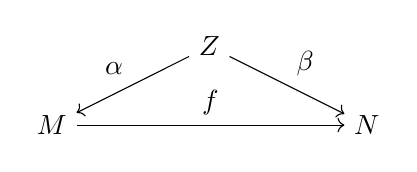
\begin{tikzpicture}
\node (Z) at (2,1) [] {$Z$};
\node (M) at (0,0) [] {$M$};
\node (N) at (4,0) [] {$N$};

\draw [->] (M) -> (N) node[midway, above] {$f$};
\draw [->] (Z) -> (M) node[midway, above left] {$\alpha$};
\draw [->] (Z) -> (N) node[midway, above right] {$\beta$};
\end{tikzpicture}
\end{center}
Ist $\beta$ glatt und $\alpha$ surjektiv und submersiv, so ist $f$ glatt. Ist $\beta$ zusätzlich submersiv, so ist es auch $f$. Ist $\beta$ zusätzlich surjektiv, so ist es auch $f$.
\begin{Beweis}{}
Sei $m \in M$ und $s : U \pfeil{} Z$ ein glatter Schnitt von $\alpha$ in einer Umgebung $U$ von $m$. Dann gilt auf $U$
\[ f =  f\circ \alpha \circ s = \beta \circ s \]
Ergo ist $f$ lokal glatt.
\end{Beweis}

\Kor{}
Sei $p : M \pfeil{} N$ eine surjektive Abbildung von Mengen. Besitzt $M$ die Struktur einer glatten Mannigfaltigkeit, so gibt es auf $N$ höchstens eine glatte Struktur, durch die $p$ zu einer Submersion wird.

\Prop{}
Sei $f : M \pfeil{} N$ eine differenzierbare Abbildung von Mannigfaltigkeiten. Definiere den \df{Graph} von $f$ durch
\[G(f) := \set{ (x,y) \in M\times N }{y = f(x)}\]
Dann ist $G(f)$ eine abgeschlossene Untermannigfaltigkeit von $M\times N$.

\Def{}
Seien $S,S' \subset M$ glatte Untermannigfaltigkeiten. Wir sagen, $S$ und $S'$ \df{schneiden sich transversal}, falls für alle $p \in S\cap S'$ gilt
\[ T_pM = T_pS + T_pS' \]
Ist noch allgemeiner eine glatte Abbildung $f : N \pfeil{} M$ gegeben, so sagen wir $f$ \df{schneidet $S$ transversal}, falls für alle $p \in f\i(S)$ gilt
\[ T_{f(p)}M = T_{f(p)}S + \d f_{p} T_pN  \]

\Prop{}
Seien Mannigfaltigkeiten $S \subset M$ und $N$ gegeben. Wird $S$ von $f : N \pfeil{} M$ transversal geschnitten, so ist $f\i(S) \subset N$ eine Untermannigfaltigkeit, die dieselbe Kodimension wie $S \subset M$ besitzt. 
\begin{Beweis}{}
Es bezeichne $k$ die Kodimension von $S \subset M$. Für ein $x\in f\i(S)$ können wir eine Umgebung $f(x) \in U \subset M$ finden, sodass $U\cap S = \phi\i(0)$ sich als Stufenmenge einer Submersion $\phi : U \pfeil{} \R^k$ darstellen lässt.\\
Es genügt nun zu zeigen, dass $\phi \circ f$ regulär in $0$ ist, da
\[ f\i(S \cap U) = f\i(\phi\i (0) \cap S) \]
Seien $z\in T_0\R^k$ und $p\in (\phi \circ f)\i(0)$. Da $\phi$ eine Submersion ist, existiert ein $y \in T_{f(p)}M $ mit
\[ \d\phi_{f(p)}(y) = z \]
Da $f$ transversal zu $S$ liegt, gibt es $y_0 \in T_{f(p)}S$ und $v \in T_pN$ mit
\[ y = y_0  + \d f_p v\]
$\phi$ ist konstant auf $S\cap U$, ergo gilt
\[ z = \d\phi_{f(p)}(y) =\d\phi_{f(p)}( y_0  + \d f_p v) = \d\phi_{f(p)}( y_0 ) +\d\phi_{f(p)}(  \d f_p v) = 0 +\d\phi_{f(p)}(  \d f_p v)
= \d(\phi\circ f)_{p}(v)  \]
Ergo ist $\d(\phi\circ f)_{p}$ surjektiv, ergo ist $\phi \circ f$ regulär in $0$.
\end{Beweis}

\Kor{}
Seien $S\subset M$ und $N$ glatte Mannigfaltigkeiten. $S \subset M$ habe Kodimension $k$.
\begin{enumerate}[1.)]
\item Ist $f : N \pfeil{} M$ eine Submersion, so ist $f\i(S) \subset N$ eine Untermannigfaltigkeit der Kodimension $k$.
\item Ist $S' \subset M$ eine Untermannigfaltigkeit der Kodimension $k'$, die $S$ transversal schneidet, so ist $S \cap S' \subset M$ eine Untermannigfaltigkeit der Kodimension $k + k'$.
\end{enumerate}

\Def{}
Für eine Äquivalenzrelation $R$ auf einer glatten Mannigfaltigkeit $M$ nennen wir $M/R$ eine \df{glatte Mannigfaltigkeit}, falls
\[  M \Pfeil{} M/R \]
eine glatte Submersion ist.

\Satz{Godement}
Sei $R$ eine Äquivalenzrelation auf einer glatten Mannigfaltigkeit $M$.\\
$M/R$ ist genau dann eine glatte Mannigfaltigkeit, wenn ist $R\subset M \times M$ eine abgeschlossene Untermannigfaltigkeit und die Projektionen
\[ p_i : R \Pfeil{} M \text{ für }i=1,2 \]
surjektive Submersionen sind.
\begin{Beweis}{}
Die Implikation nach rechts ist klar.\\
Betrachte für die andere Richtung folgende Lemmata, die alle unter der Voraussetzung gelten, dass $R \subset M\times M$ abgeschlossen und $p_i$ surjektive Submersionen sind.
\Lem{1}
$M \pfeil{} M/R$ ist offen und ergo $M/R$ hausdorffsch.
\Lem{2}
Jede Äquivalenzklasse von $R$ ist eine abgeschlossene Untermannigfaltigkeit der Dimension $\dim R - \dim M$.
\Lem{3}
Für jedes $a \in M$ existiert eine offene Umgebung $a \in U \subset_o M$ mit einer abgeschlossenen Mannigfaltigkeit $S \subset U$ und einer Submersion $q:U \pfeil{} S$, sodass für jedes $x \in U$ gilt
\[ [x]\cap U \cap S = \{q(x)\} \]
$S$ nennt man in diesem Fall einen \df{Schnitt durch die Äquivalenzklassen von $R$} in $U$.

% % %Ls zehnte
\Def{}
Ist $V \subset M$ eine Teilmenge, so setze $R_V := (V \times V)\cap R$
\Kor{}
Sei $a\in M$, dann existiert eine offene Umgebung $a \in U \subset_oM$, sodass $U \pfeil{} U/R_U$ eine surjektive Submersion von glatten Mannigfaltigkeiten ist.
\Def{}
$V\subset M$ heißt \df{saturiert}, wenn sich $V$ als die Vereinigung von Äquivalenzklassen darstellen lässt, d.\,h.
\[ V = \pi_R\i (\pi_R(V)) \]
\Lem{4}
Sei $a \in M$, dann existiert eine offene Umgebung $a \in U \subset_oM$, sodass $U \pfeil{} U/R_U$ eine surjektive Submersion von glatten Mannigfaltigkeiten ist. Setzt man $V := \pi_R\i (\pi_R(U))$, so ist $V \pfeil{} U/R_U$ eine surjektive Submersion.
\Kor{}
In obiger Situation ist $V/R_V$ eine glatte Mannigfaltigkeit.
\Kor{}
Jeder Punkt ist in einer saturierten offenen Nachbarschaft $V$ enthalten, sodass $V \pfeil{} V/R_V$ eine surjektiv Submersion glatter Mannigfaltigkeiten ist.
\end{Beweis}

\newpage
\section{Lie-Gruppen und Überlagerungen}
\Def{Lie-Gruppe}
Eine \df{Lie-Gruppe} ist eine glatte Mannigfaltigkeit $G$, die eine Gruppenstruktur trägt, deren Multiplikation $G \times G \pfeil{} G$ und Inversion $G \pfeil{} G$ glatte Abbildungen sind.

\Lem{}
Sei $G \curvearrowright M$ die stetige Wirkung einer beliebigen Gruppe auf einer Mannigfaltigkeit $M$. Dann ist $M\pfeil{}M/G$ offen.

\Kor{}
$M/G$ ist genau dann hausdorffsch, wenn die Abbildung
\begin{align*}
M \times G & \Pfeil{} M \times M\\
(x, g) & \longmapsto (x, g.x)
\end{align*}
ein abgeschlossenes Bild hat.

\Def{}
Eine Gruppenwirkung $G\curvearrowright M$ heißt \df{frei}, wenn für jedes $m \in M$ der \df{Stabilisator}
\[ Stab_G(m) = \set{g \in G}{m.g = m} \]
trivial ist. Die Wirkung heißt \df{eigentlich}, falls die Abbildung
\begin{align*}
G \times M & \Pfeil{} M \times M\\
(g,m) & \longmapsto (m, m.g)
\end{align*}
eigentlich ist, d.\,h., das Urbild kompakter Mengen ist wieder kompakt.

\Def{}
Ein Vektorfeld $V$ auf einer Lie-Gruppe heißt \df{rechts-invariant}, falls für alle $g \in G$
\[ \d R_g(V) = V \]
gilt, wobei $R_g : p \mapsto pg$ die Rechtsmultiplikation mit $g$ bezeichnet. Mit $\V_R(G) \subset \V(G)$ fassen wir den Vektorraum aller rechts-invarianten Vektorfelder zusammen.\\
Definiere ferner die {Lie-Algebra} von $G$ durch
\[ \g := T_eG \]
so existiert für jedes $X \in \g$ genau ein rechts-invariantes Vektorfeld $X^R := g\mapsto \d R_g(X)$ mit
\[ X^R (e) = X \]
Wir erhalten hierdurch einen linearen Isomorphismus
\begin{align*}
\g &\Pfeil{} \V_R(G)\\
X & \longmapsto X^R
\end{align*}
Da es sich bei $\V_R(G) \subset \V(G)$ um eine Lie-Subalgebra handelt, erhalten wir durch diesen Isomorphismus eine Lie-Algebrenstruktur auf $\g$. Zusammen mit dieser Struktur nennen wir $\g$ die \df{Lie-Algebra der Lie-Gruppe $G$}.\\
Unter einer \df{Ein-Parameter-Untergruppe} verstehen wir einen Gruppenhomomorphismus $\R \pfeil{} G$. Für jedes $X \in \g$ existiert genau eine Ein-Parameter-Untergruppe
\begin{align*}
\alpha_X : \R \Pfeil{} G
\end{align*}
mit $\dot{\alpha_X}(0) = X$. Wir definieren hierdurch folgende \df{Exponentialabbildung}
\begin{align*}
\text{Exp} : \g & \Pfeil{} G\\
X & \longmapsto \alpha_X(1)
\end{align*}
Diese ist glatt und es gilt
\begin{align*}
\alpha_X(t) &= \text{Exp}(tX)\\
\text{Exp}(tX) \circ \text{Exp}(sX) &= \text{Exp}((t+s)X)\\
\frac{\d}{\d t} \text{Exp}(tX)_{|t= 0} = X
\end{align*}
Jedes $X \in \g$ induziert ein glattes Vektorfeld $X^*$ auf $G$ durch
\[ X^*(p) := \frac{\d}{\d t} p \cdot \text{Exp}(tX)_{|t = 0} \]

\Satz{}
Sei $G \curvearrowright M$ die glatte, freie und eigentlich Wirkung einer Lie-Gruppe auf einer glatten Mannigfaltigkeit. Dann besitzt $M/G$ genau eine Struktur einer glatten Mannigfaltigkeit durch die $M\pfeil{} M/G$ zu einer glatten Submersion wird.
\begin{Beweis}{}
Betrachte folgende Abbildung
\begin{align*}
\alpha : M \times G & \Pfeil{} M \times M\\
(x,g) & \longmapsto (x, g.x)
\end{align*}
Um Godements Satz anzuwenden, müssen wir zeigen, dass $\alpha$ die Einbettung einer abgeschlossenen Untermannigfaltigkeit ist, und, dass die Projektionen $p_i : R \pfeil{} M$ submersiv sind.\\
Seien $x \in M,g\in G$ und $X,Y\in \V(M)$, so gilt
\begin{align*}
\d \alpha_{(x,g)}(X,(\d L_g)_e Y) &= \d \alpha_{(x,g)}(X,0) +\d \alpha_{(x,g)}(0,(\d L_g)_e Y)\\
&= \d \alpha(\gamma(t),g)_{|t = 0} +\d \alpha(x,( L_g(\text{Exp}(tY))))_{|t = 0}\\
&= \d (\gamma(t),R_g(\gamma(t))_{|t = 0} +\d (x,( xg\text{Exp}(tY)))_{|t = 0}\\
&=  (X,R_g(X)) + (0,Y^*(xg))\\
\end{align*}
wobei $\gamma : I \pfeil{} M$ eine Geodäte mit $\gamma(0) = x$ und $\dot{\gamma}(0) = X$ ist.\\
Da $G\curvearrowright M$ frei ist, sind $\alpha$ und $\d \alpha$ injektiv, ergo handelt es sich bei $\alpha$ um eine Immersion.\\
Die Projektionen sind nun submersiv, da gilt
\[p_1 \circ \alpha(m,g) = m \]
\end{Beweis}

% % %LS elfte
\Def{Faserbündel}
Es seien $E,F,B$ glatte Mannigfaltigkeiten. Ein \df{Faserbündel} über einer \df{Basis} $B$ mit \df{Faser} $F$ und \df{Totalraum} $E$ ist eine surjektive Submersion
\[ p : E \pfeil{} B \]
die \df{lokal trivial} ist, d.\,h., für jeden Punkt $x \in B$ existiert eine Umgebung $x\in U \subset_o B$ und ein Diffeomorphismus
\[ \phi_U : p\i(U) \Pfeil{} U \times F \]
sodass folgendes Diagramm kommutiert
\begin{center}
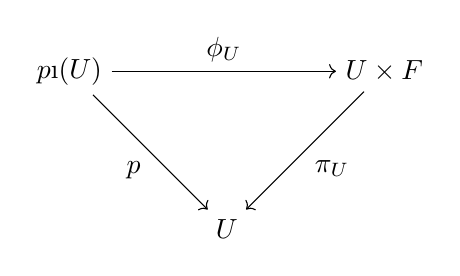
\begin{tikzpicture}
\node (pU) at (0,2) [] {$p\i(U)$};
\node (UF) at (4,2) [] {$U \times F$};
\node (U) at (2,0) [] {$U$};

\draw [->] (pU) -> (UF) node[midway, above] {$\phi_U$};
\draw [->] (pU) -> (U) node[midway, below left] {$p$};
\draw [->] (UF) -> (U) node[midway, below right] {$\pi_U$};
\end{tikzpicture}
\end{center}
Insbesondere ist $p\i(x)$ diffeomorph zur Faser $F$.\\
Existiert sogar ein Diffeomorphismus $\phi_B$, der folgendes Diagramm kommutieren lässt
\begin{center}
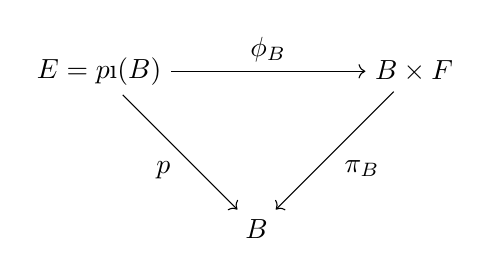
\begin{tikzpicture}
\node (pU) at (0,2) [] {$E = p\i(B)$};
\node (UF) at (4,2) [] {$B \times F$};
\node (U) at (2,0) [] {$B$};

\draw [->] (pU) -> (UF) node[midway, above] {$\phi_B$};
\draw [->] (pU) -> (U) node[midway, below left] {$p$};
\draw [->] (UF) -> (U) node[midway, below right] {$\pi_B$};
\end{tikzpicture}
\end{center}
so spricht man von einem \df{trivialen Faserbündel.}

\Def{Hauptfaserbündel}
Sei $G$ eine Lie-Gruppe und $B$ eine glatte Mannigfaltigkeit. Ein \df{Hauptfaserbündel} mit \df{Strukturgruppe} $G$ über $B$ ist ein Faserbündel $p:M \pfeil{} B$ mit Faser $G$ und einer glatten Rechtswirkung $G\curvearrowright M$, sodass für jedes $x\in B$ eine Umgebung $x \in U \subset_o B$ und ein Diffeomorphismus
\[ \tau : p\i(U) \Pfeil{} U \times G \]
existiert, durch die die Wirkung durch $G$ trivial wird, d.\,h., folgendes Diagramm kommutiert
\begin{center}
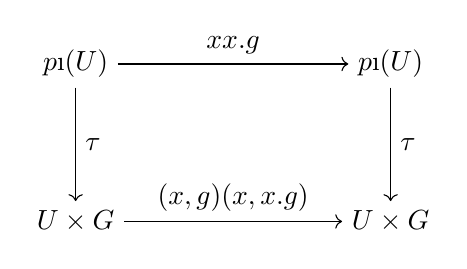
\begin{tikzpicture}
\node (pU1) at (0,2) [] {$p\i(U)$};
\node (pU2) at (4,2) [] {$p\i(U)$};
\node (UG2) at (4,0) [] {$U \times G$};
\node (UG1) at (0,0) [] {$U \times G$};

\draw [->] (pU1) -> (pU2) node[midway, above] {$x \pfeil{} x.g$};
\draw [->] (UG1) -> (UG2) node[midway, above] {$(x,g) \pfeil{} (x, x.g)$};
\draw [->] (pU1) -> (UG1) node[midway, right] {$\tau$};
\draw [->] (pU2) -> (UG2) node[midway, right] {$\tau$};
\end{tikzpicture}
\end{center}

\Satz{}
\begin{enumerate}[1.)]
\item Sei $G\curvearrowright M$ die glatte, freie und eigentliche Wirkung einer Lie-Gruppe auf einer Mannigfaltigkeit $M$. Dann besitzt $M/G$ genau eine Mannigfaltigkeitstruktur, durch die $M \pfeil{} M/G$ zu einer Submersion wird. Ferner ist $M\pfeil{} M/G$ in diesem Fall ein Hauptbündel mit Strukturgruppe $G$.
\item Sei $p : M \pfeil{} B$ ein Hauptbündel mit Strukturgruppe $G$. Dann wirkt $G$ frei und eigentlich auf $M$ und $p$ faktorisiert über einen Diffeomorphismus $M/G \pfeil{\sim} B$.
\end{enumerate}

\newpage
\section{Schall und Rauch}
\Def{Erinnerung}
Zwei Punkte $P,Q$ auf einer Geodäte $\gamma$ heißen \df{konjugiert} (bzgl. $\gamma$), falls ein Jacobi-Feld auf $\gamma$ existiert, das bei $P$ und $Q$ verschwindet.

\Lem{Das Index-Lemma}
Sei $M$ eine Riemannsche Mannigfaltigkeit. Für eine Geodäte $\gamma : [0,a] \pfeil{} M$ und ein stückweise glattes Vektorfeld $V$ entlang $\gamma$, setzen wir
\[ I_{t_0}(V,V) = \int_{0}^{t_0} \klam{ g(\D_tV, \D_tV) - g(\Rc(\dot{\gamma}, V)\dot{\gamma}, V ) } \d t \]
für $t_0 \in [0,a]$. Liegt nun auf $\gamma_{|(0,a]}$ kein Punkt, der zu $\gamma(0)$ konjugiert ist und sind ein beliebiges stückweise glattes Vektorfeld $V$ und ein Jacobi-Feld $J$ auf $\gamma$ gegeben, die beide orthogonal zu $\dot{\gamma}$ stehen, d.\,h.
\[ g(J, \dot{\gamma}) = 0 = g(V, \dot{\gamma}) \]
die ferner auch beide in $\gamma(0)$ verschwinden, d.\,h.
\[ J(0) = V(0) = 0 \]
und in einem weiteren Punkt übereinstimmen, d.\,h., es gibt ein $t_0\in (0,a]$, s.\,d.
\[ J(t_0) = V(t_0) \]
so gilt
\[ I_{t_0}(J,J) \leq I_{t_0} (V,V) \]
wobei Gleichheit genau dann gilt, wenn $J$ und $V$ auf $[0,t_0]$ übereinstimmen.

\begin{Beweis}{}
Der Raum aller Jacobi-Felder auf $\gamma$, die in $\gamma(0)$ verschwinden und orthogonal zu $\dot{\gamma}$ stehen, besitzt Dimension $n-1$, wobei $n = \dim M$. Dementsprechend wählen wir eine Basis $J_1,\ldots, J_{n-1}$ dieses Raumes, und erhalten Skalare $a_i \in \R$, mit denen gilt
\[ J = \sum_{i = 1}^{n-1} a_i J_i \]
Da auf $(0,a]$ keine zu $\gamma(0)$ adjungierten Punkte existieren, bilden die $J_i$ eine Basis von $\dot{\gamma}(t)^\bot \subset T_\gamma M$.\\
Ergo existieren stückweise glatte Funktionen $f_i : [0,a] \pfeil{} \R$, sodass
\[ V = \sum_{i = 1}^{n-1}f_i J_i \]
Wir wollen nun folgende Gleichung zeigen
\begin{align*}
\tag{1}
g(\D_tV, \D_tV) - g(\Rc(\dot{\gamma}, V)\dot{\gamma}, V) 
=
g\klam{ \sum_{i = 1}^{n-1} f_i' J_i, \sum_{i = 1}^{n-1} f_i' J_i }
+ \frac{\d}{\d t} g
\klam{ \sum_{i = 1}^{n-1} f_i J_i, \sum_{i = 1}^{n - 1} f_i D_tJ_i }
\end{align*}
Tatsächlich gilt
\begin{align*}
& g(\D_tV, \D_tV) - g(\Rc(\dot{\gamma}, V)\dot{\gamma}, V) \\
=&
g( \sum_{i = 1}^{n-1} f_i'J_i + f_i\D_tJ_i, \sum_{i = 1}^{n-1} f_i'J_i + f_i\D_tJ_i )
-
g(\sum_{i=1}^{n-1} f_i \Rc(\dot{\gamma}, J_i)\dot{\gamma}, \sum_{i = 1}^{n-1}f_i J_i )\\
=& g( \sum_{i = 1}^{n-1} f_i'J_i + f_i\D_tJ_i, \sum_{i = 1}^{n-1} f_i'J_i + f_i\D_tJ_i )
-
g(\sum_{i=1}^{n-1} f_i \cdot (-\D_t\D_t J_i), \sum_{i = 1}^{n-1}f_i J_i )
\end{align*}
und
\begin{align*}
& \frac{\d}{\d t} g \klam{ \sum_{i=1}^{n-1} f_i J_i, \sum_{i = 1}^{n-1} f_i \D_t J_i }\\
= & g \klam{ \sum_{i=1}^{n-1} f_i' J_i + f_i D_t J_i, \sum_{i = 1}^{n-1} f_i \D_t J_i }
+g \klam{ \sum_{i=1}^{n-1} f_i J_i, \sum_{i = 1}^{n-1} f_i' \D_t J_i + f_i \D_t\D_t J_i }
\end{align*}
D.\,h., Gleichung (1) ist äquivalent zu folgender Gleichung
\begin{align*}
\tag{2}
g\klam{\sum_{i = 1}^{n-1} f_i \D_t J_i, \sum_{i = 1}^{n-1} f_i' J_i} 
= 
g\klam{\sum_{i = 1}^{n-1} f_i J_i , \sum_{i = 1}^{n-1} f_i' \D_t J_i }
\end{align*}
Um Gleichung (2) zu zeigen, legen wir folgende Funktion fest
\[ h(t) := g(\D_t J_i, J_j)(t) - g(J_i, \D_t J_j)(t) \]
dann gilt
\begin{align*}
h(0) =& 0\\
{h}'(t) =& \frac{\d}{\d t}(g(\D_t J_i, J_j)(t) - g(J_i, \D_t J_j)(t))\\
=& g(\D_t\D_t J_i, J_j)(t) +  g(\D_t J_i, \D_t J_j)(t) - g(\D_tJ_i, \D_t J_j)(t) -g(J_i, \D_t\D_t J_j)(t)\\
=& g(\Rc(\dot{\gamma}, J_i) \dot{\gamma}, J_j)(t) - g(J_i, \Rc(\dot{\gamma}, J_j) \dot{\gamma} )\\
\gl{Blockvertauschung}& g(\Rc(\dot{\gamma}, J_j) \dot{\gamma}, J_i)(t) - g(J_i, \Rc(\dot{\gamma}, J_j) \dot{\gamma} ) = 0
\end{align*}
ergo $h(t) = 0$ und damit einhergehend
\[ g(\D_t J_i, J_j) = g(J_i, \D_t J_j) \]
Dadurch folgt insbesondere Gleichung (2) und Gleichung (1).\\
Mithilfe von Gleichung (1) folgt nun
\begin{align*}
I_{t_0}(V,V) =& \int_{0}^{t_0} \klam{ g(\D_tV, \D_tV) - g(\Rc(\dot{\gamma}, V)\dot{\gamma}, V ) } \d t \\
=&\int_{0}^{t_0} \klam{ g\klam{ \sum_{i = 1}^{n-1} f_i' J_i, \sum_{i = 1}^{n-1} f_i' J_i }
+ \frac{\d}{\d t} g
\klam{ \sum_{i = 1}^{n-1} f_i J_i, \sum_{i = 1}^{n - 1} f_i D_tJ_i } } \d t \\
=&\int_{0}^{t_0}  g\klam{ \sum_{i = 1}^{n-1} f_i' J_i, \sum_{i = 1}^{n-1} f_i' J_i } \d t
+
g\klam{ \sum_{i = 1}^{n-1} f_i J_i, \sum_{i = 1}^{n - 1} f_i D_tJ_i } (t_0)\\
\gl{(*)}&\int_{0}^{t_0}  \norm{\sum_{i = 1}^{n-1} f_i' J_i}^2 \d t
+
g\klam{ \sum_{i = 1}^{n-1} a_i J_i, \sum_{i = 1}^{n - 1} a_i D_tJ_i } (t_0)\\
=& \int_{0}^{t_0}  \norm{\sum_{i = 1}^{n-1} f_i' J_i}^2 \d t
+ I_{t_0}(J,J)
\\
\geq & I_{t_0} (J,J)
\end{align*}
Beachte, dass $f_i(t_0) = a_i$ bei $(*)$ gilt, da $J(t_0) = V(t_0)$.\\
Gilt nun
\[ I_{t_0}(J,J) = I_{t_0}(V,V) \]
so folgt
\[ \sum_{i = 1}^{n-1}f'_i J_i = 0 \]
Da die $J_i$ auf $(0,a]$ linear unabhängig sind, folgt $f_i' = 0$, d.\,h., die $f_i$ sind konstant gleich $a_i$ und $J = V$.
\end{Beweis}

\Satz{Rauch}
Seien $M, \l M$ Mannigfaltigkeiten der Dimension $n$ bzw. $n + k$. Seien ferner $\gamma : I \pfeil{}M $ und $\l \gamma : I \pfeil{} \l M$ Geodäten derselben Geschwindigkeit. Ferner soll $\l \gamma(0)$ keinen konjugierten Punkt auf $\l \gamma (0,a]$ haben und für alle $x \in T_{\gamma(t)} M$ und $y \in T_{\l \gamma (t)} \l M$ soll gelten
\[ \kappa(x, \dot{\gamma}(t)) \leq \l\kappa(y, \dot{\l \gamma}(t)) \] 
Sind ferner Jacobifelder $J,\l J$ entlang $\gamma$ bzw. $\l \gamma$ gegeben, dergestalt, dass $J(0), \l J(0)$ tangential zu $\gamma$ bzw. $\l \gamma$ sind und
\begin{align*}
\norm{J(0)} = \norm{\l J(0)} \text{, } \norm{\D_tJ(0)} = \norm{\l \D_t \l J(0)} \text{ und } g(\D_t J(0),\dot{\gamma}(0)) = g(\l\D_t\l J(0), \dot{\l \gamma}(0))
\end{align*}
gelten, so folgt
\[ \norm{\l J(t)} \leq \norm{J(t)} \]

\begin{Beweis}{}
\begin{itemize}
\item Wir nehmen zuerst an, dass folgende Dinge gelten
\[ \norm{J(0)} = g(\D_t J(0), \dot{\gamma}(0)) = 0 \text{ und } \norm{\l J(0)} = g(\l \D_t \l J(0), \dot{\l \gamma}(0)) = 0 \]
Hieraus folgt, dass $J,\l J$ orthogonal auf $\gamma$ bzw. $\l \gamma$ stehen, denn, da $\gamma$ eine Geodäte ist, gilt
\[ g(J(t), \dot{\gamma}(t)) = t \cdot g(\D_tJ(0), \dot{\gamma}(0)) + g(J(0), \dot{\gamma}(0)) \]
Gilt nun
\[ \norm{D_t J(0)} = \norm{\l D_t \l J(0)} = 0 \]
so folgt sofort
\[\norm{J(t)} = \norm{\l J(t)} = 0 \]
Anderenfalls setze
\[ v(t) := \norm{J(t)}^2 \text{ und } \l v(t) = \norm{\l J(t)}^2 \]
Da $\l \gamma(0,a]$ keine konjugierten Punkte hat, ist $\frac{v(t)}{\l v(t)}$ wohldefiniert auf $(0,a]$. Es folgt
\[ \lim_{t \pfeil{} 0} \frac{v(t)}{\l v(t)} = \lim_{t \pfeil{} 0} \frac{\ddot{v}(t)}{\ddot{\l{v}}(t)} = \frac{\norm{\D_tJ(0)}^2}{\norm{\l \D_t \l J(0)}^2} = 1 \] 
Um zu zeigen, dass $\frac{v(t)}{\l v(t)} \geq 1$, genügt es
\[ \frac{\d}{\d t} (\frac{v(t)}{\l v(t)}) \geq 0 \]
zu zeigen, was gerade äquvialent ist zu
\[ \tag{1} \dot{v}(t) \l v(t) \geq v(t) \dot{\l v}(t) \]
Fixiere hierzu $t_0 \in (0,a]$. Gilt gerade $v(t_0) = 0$, so folgt auch
\[ \dot{v}(t_0) = 2g(\D_t J(t_0), J(t_0) = 0\]
und (1) gilt für $t = t_0$.\\
Sei also $v(t_0), \l v(t_0) \neq 0$, man setze
\[ U := \frac{1}{\sqrt{v(t_0)}}J \text{  und  } \l U :=  \frac{1}{\sqrt{\l v(t_0)}}\l J  \]
Dann folgt
\begin{align*}
\frac{\dot{v}(t_0)}{v(t_0)} =&\frac{2g(\D_tJ(t_0), J(t_0)}{v(t_0)}\\
=& 2g(\D_t U(t_0), U(t_0)\\
=& \frac{\d}{\d t}g(U,U)_{|t = t_0}\\
=& \int_{0}^{t_0} \frac{\d^2}{\d t^2}g(U,U) \d t\\
=& 2\int_{0}^{t_0} \klam{ g(\D_t U, \D_t U)  + g(U, \D_t \D_t U) } \d t\\
=& 2\int_{0}^{t_0} \klam{ g(\D_t U, \D_t U)  + g(U, - \Rc(\dot{\gamma}, U) \dot{\gamma} ) } \d t\\
=& I_{t_0}(U,U)
\end{align*}
und analog
\begin{align*}
\frac{\dot{\l v}(t_0)}{\l v(t_0)} =I_{t_0}(\l U,\l U)
\end{align*}
Ergo folgt (1) aus folgender Ungleichung
\[ I_{t_0}(U,U) \geq I_{t_0}(\l U, \l U) \]
Es seien nun folgende parallelen ONBs entlang $\gamma$ bzw. $\l \gamma$ gegeben
\begin{align*}
e_1 = \frac{\dot{\gamma}}{\norm{\dot{\gamma}}}, e_2, e_3, \ldots, e_{n} \text{ und } \l e_1 = \frac{\dot{\l\gamma}}{\norm{\dot{\l\gamma}}}, \l e_2 , \l e_3,\ldots, \l e_{n+k}
\end{align*}
mit
\[ e_2(t_0) = U(t_0) \text{ und } \l e_2(t_0) = \l U (t_0) \]
Definiere dann folgende Abbildung
\begin{align*}
\Phi : \V_\gamma &\Pfeil{} \V_{\l \gamma}\\
\sum_{i = 1}^{n} f_i e_i &\longmapsto \sum_{i = 1}^{n} f_i \l e_i
\end{align*}
Für diese gilt
\begin{align*}
g(\Phi V, \Phi V) = g(V,V) \text{ und } \l \D_t(\Phi V) = \Phi (\D_t V)
\end{align*}
Man rechnet nach
\begin{align*}
I_{t_0}(\Phi U, \Phi U) \leq ... = I_{t_0}(U, U)
\end{align*}
$\l U$ und $\Phi U$ erfüllen nun beide die Voraussetzungen des Index-Lemmas, weswegen folgt
\[ I_{t_0}(\l U, \l U) \leq I_{t_0} ( \Phi U, \Phi U) \]
Ergo folgt in diesem Fall die Behauptung.
\item Gelten die Voraussetzungen des ersten Falles nicht, so zerlege
\[ J = J^\bot + \frac{g(J,\dot{\gamma})}{g(\dot{\gamma},\dot{\gamma})} \dot{\gamma} \text{ und } 
 \l J = \l{J}^\bot + \frac{g(\l J,\dot{\l\gamma})}{g(\dot{\l\gamma},\dot{\l\gamma})} \dot{\l\gamma}\] 
Dann gilt laut erstem Fall
\[ \norm{\l{ J}^\bot} \leq \norm{J^\bot} \]
und deswegen
\[ \norm{\l{ J}} \leq \norm{J} \]
da 
\begin{align*}
g(J, \dot{\gamma}) &= g(\D_t J(0), \dot{\gamma}(0))t + g(J(0), \dot{\gamma})(0)\\
&= g(\l\D_t \l J(0), \dot{\l\gamma}(0))t + g(\l J(0), \dot{\l\gamma})(0)\\
&= g(\l J, \dot{\l \gamma})
\end{align*}
\end{itemize}
\end{Beweis}

% %Ls zwölfte
\Bem{Erinnerung}
Sei $M$ eine Riemannsche Mannigfaltigkeit konstanter Schnittkrümmung $\kappa$ und sei $\gamma:[0,l]\pfeil{}M$ eine nach Bogenlänge parametrisierte Geodäte.\\
Ein Jacobi-Feld entlang $\gamma$ orthogonal zu $\dot{\gamma}$ kann anhand einer Basis paralleler Vektorfelder $e_1,\ldots, e_{n-1} \in \dot{\gamma}^\bot$ ausgedrückt werden durch
\begin{align*}
J(t) = 
\left\lbrace
\begin{aligned}
\sum_{i= 1}^{n-1} (a_i \sin(\sqrt{\kappa} \cdot t) + b_i \cos (\sqrt{\kappa}\cdot  t) ) e_i(t) && \kappa > 0\\
\sum_{i= 1}^{n-1} (a_it + b_i ) e_i(t) && \kappa = 0\\
\sum_{i= 1}^{n-1} (a_i \sinh(\sqrt{-\kappa}\cdot t) + b_i \cosh (\sqrt{-\kappa} \cdot t) ) e_i(t) && \kappa < 0
\end{aligned}
\right.
\end{align*}
Ist $\kappa \leq 0$, so besitzen Geodäten keine konjugierten Punkte. Ist $\kappa > 0$, so tauchen konjugierte Punkte in Abständen von $\frac{\pi}{\sqrt{\kappa}}$ auf.

\Kor{}
Sei $M$ eine Riemannsche Mannigfaltigkeit deren Schnittkrümmung $\kappa$ begrenzt wird durch konstante Schranken
\[ 0 \leq l \leq \kappa(v,w) \leq h \]
Ist $\gamma$ eine Geodäte auf $M$, so liegt der Abstand $d$ zwischen zwei konjugierten Punkten auf $\gamma$ zwischen
\[ \frac{\pi}{\sqrt{h}} \leq d \leq \frac{\pi}{\sqrt{l}} \]

\Bem{Erinnerung}
Sei $\gamma$ eine nach Bogenlänge parametrisierte Geodäte. Dann sind Punkte $p = \gamma(t_0)$ und $q = \gamma(t_1)$ genau dann konjugiert, wenn $(t_1 - t_0)\cdot\dot{\gamma}(t_0)$ ein \df{kritischer} bzw. \df{singulärer} Punkt von $\exp_p$ ist, d.\,h. die Abbildung
\[ \d (\exp_p)_{(t_1 - t_0)\cdot\dot{\gamma}(t_0)} : T_pM  \Pfeil{} T_qM \]
ist kein Isomorphismus.

\Kor{}
Seien Riemannsche Mannigfaltigkeiten $M, \l M$ der Dimensionen $n$ bzw. $n + k$ gegeben. Ferner sei die Schnittkrümmung $\l \kappa$ von $\l M$ stets größer als die Schnittkrümmung $\kappa$ von $M$.\\
Seien $p\in M, \l p \in \l M$ und $r > 0$, sodass ${\exp_p}_{| B_r(0)}$ eine Einbettung und ${\exp_{\l p}}_{|B_r(0)}$ nicht-singulär ist. Sei ferner
\[ i : T_pM \Inj{} T_{\l p}\l M\]
eine lineare, injektive Abbildung, die die Metrik erhält, und
\[c : [0,a] \Pfeil{} \exp_p(B_r(0))\]
eine glatte Kurve. Für die glatte Kurve
\[ \l c := \exp_{\l p} \circ i\circ  \exp_p\i \circ c : [0,a]  \Pfeil{} \exp_{\l p}(B_r(0)) \]
gilt nun
\[ L(\l c) \leq L(c) \]
\begin{Beweis}{}
Definiere folgende Kurve in $T_pM$
\[ \widetilde{c} := \exp_p\i \circ c \]
und folgende Abbildung
\[ f(t,s) := \exp_{p}(t\widetilde{c}(s)) \]
Dann ist für alle $s$ folgendes Jacobi-Feld entlang einer Geodäte $\gamma_s(t) := f(t,s)$ gegeben
\[ J_s(t) := \frac{\d}{\d s} f(t,s) = (\d \exp_p)_{t\widetilde{c}(s)}(t\dot{\widetilde{c}}(s)) \]
Betrachten wir analog
\[ \l f(t,s) := \exp_{\l p}(t i(\widetilde{c}(s))) \]
so erhalten wir analog Jacobi-Felder entlang Geodäten $\l\gamma_s(t) := \l f(t,s)$
\[ \l J_s(t) := \frac{\d}{\d s}f(t,s)\]
Mit Rauchs Satz erhalten wir nun
\[ \norm{\dot{\l c}(s)} = \norm{\l J_s(1)} \leq \norm{J_s(1)} = \norm{\dot{c}(s)} \]
\end{Beweis}

\Kor{Satz von Cartan-Hadamard}
Sei $M$ eine vollständige und wegzusammenhängende Mannigfaltigkeit nicht-positiver Schnittkrümmung. Dann ist
\[ \exp_p :T_pM \pfeil{} M \]
eine Überlagerung.

\Def{}
Zwei geschlossene Pfade $\gamma_1, \gamma_2 : S^1 \pfeil{} M$ heißen \df{frei homotop}, falls eine freie Homotopie $H : S^1 \times [0,1] \pfeil{} M$ existiert mit
\[ H(t,0) = \gamma_1(t) \text{ und } H(t,1) = \gamma_2(t) \]
Unter $C_1(M)$ verstehen wir die Menge aller Äquivalenzklassen der freien Homotopie. Wir erhalten eine natürliche Abbildung
\[ \Phi : \pi_1(M,p) \Pfeil{} C_1(M) \]
Ist $M$ wegzusammenhängend, so ist $\Phi$ surjektiv. Ferner stimmen die Bilder von zwei Klassen aus $C_1(M)$ genau dann überein, wenn sie konjugiert in $\pi_1(M,p)$ sind. Ergo liefert $\Phi$ eine Bijektion zwischen $C_1(M)$ und $\pi_1(M,p)/Konjugation$, wenn $M$ wegzusammenhängend ist.\\
Eine freie Homotopieklasse heißt \df{trivial}, wenn sie eine konstante Schleife enthält. Ein \df{geodätisches Lasso} ist ein geschlossener Weg, der auf allen Punkten außer einem geodätisch ist.

\Satz{Cartan}
Ist $M$ eine kompakte Riemannsche Mannigfaltigkeit, so besitzt jede nicht triviale freie Homotopieklasse eine geschlossene Geodäte.

\begin{Beweis}{}
Sei $\alpha \in C_1(M)$ eine nicht-triviale freie Homotopieklasse. Dann ist
\[ d:= \inf \set{L(c)}{c \in \alpha} > 0 \]
Sei dazu $(c_i)_i \in \alpha^\N$ eine gleichmäßig stetige Folge, deren Längen gegen $d$ konvergieren. Da $M$ kompakt ist, existiert eine Subfolge, die gegen eine gleichmäßig konvergente Schleife $\gamma^*$ konvergiert.\\
Bezeichne mit $\gamma$ eine stückweise geodätische Approximation von $\gamma^*$. Dann gilt
\[ L(\gamma) = d\]
Nun kann man sich aber auch überlegen, dass $\gamma$ bereits eine geschlossene Geodäte ist, da die Länge von $\gamma$ stückweise minimal ist.
\end{Beweis}

\Kor{}
Sei $M$ eine kompakte Riemannsche Mannigfaltigkeit. Ist $M$ nicht einfach zusammenhängend, so existiert eine geschlossene Geodäte in $M$.

\newpage
\chapter{Zweiter Teil, Geometrische Aussagen}
% % % Ws erste, 7.12.17
\section{Trigonometrie mit oberer Krümmungsschranke}
\Def{}
Ein \df{geodätisches Dreieck} $\Delta(a,b,c)$ besteht aus drei geodätischen Segmenten $a,b,c$, die sich paarweise in den Punkten $A,B,C$ schneiden. Die \df{Winkel} bei $A,B,C$ bezeichnen wir mit $\alpha, \beta, \gamma$ und geben ihnen ein Maß durch
\[ \cos(\alpha) = \frac{g_{A}(v_B,v_C)}{\norm{v_B}\norm{v_C}} \]
Die \df{Längen} von $a,b,c$ bezeichnen wir mit $\bet{a}, \bet{b}, \bet{c}$.

\Def{}
Zu einer Riemannschen Mannigfaltigkeit $M$ mit Schnittkrümmung $\leq \kappa$ sei $M^2_\kappa$ die zwei-dimensionale Mannigfaltigkeit der konstanten Schnittkrümmung $\kappa$.\\
Ist $\Delta = \Delta(a,b,c)$ ein Dreieck in $M$, so verstehen wir unter einem \df{Vergleichs-Dreieck} $\l\Delta = \l \Delta(\l a, \l b,\l c) \subset M^2_\kappa$ ein geodätisches Dreieck, das dieselben Längen besitzt, d.\,h.
\[ \bet{a} = \bet{\l a}, \bet{b} = \bet{\l b} \text{ und } \bet{c} = \bet{\l c} \]
Solch ein Vergleichs-Dreieck existiert und ist bis auf Isometrien eindeutig, falls gilt
\begin{itemize}
\item $\bet{a} + \bet{b} \geq \bet{c}$, $\bet{b} + \bet{c} \geq \bet{a}$ und $\bet{c} + \bet{a} \geq \bet{b}$
\item $\bet{a} + \bet{b} + \bet{c} < \frac{2\pi}{\sqrt{\kappa}}$, falls $\kappa > 0$  
\end{itemize}
\Bem{}
Ist $M$ eine \df{Hadamard-Mannigfaltigkeit}, d.\,h., $\kappa_M \leq 0$ und $M$ ist einfach zusammenhängend, so ist ein geodätisches Dreieck immer durch seine Eckpunkte festgelegt und ein Vergleichs-Dreieck in $M^2_0 = \R^2$ existiert immer.

\Satz{Umgekehrtes Toponogov Theorem}
\label{091216}
Sei $M$ eine Riemannsche Mannigfaltigkeit mit Schnittkrümmung $\leq \kappa$. Sei $p \in M$, $R < inj(P)$ und $R \leq \frac{\pi}{\sqrt{\kappa}}$. Sei ferner $\Delta = \Delta(a,b,c)$ ein geodätisches Dreieck in $B_p(R)$ mit $C = p$ und
\[ \bet{a} + \bet{b} + \bet{c} < \frac{2\pi}{\sqrt{\kappa}} \]
Dann folgt
\[\bet{c} \leq \bet{a} + \bet{b}\]
und für das Vergleichs-Dreieck $\l \Delta = \l \Delta(\l a, \l b, \l c) \subset M^2_\kappa$ gilt
\begin{enumerate}[(1)]
\item $d(p,q) \leq \l d(\l p, \l q)$ für alle $q \in int(c)$ und korrespondierenden Punkten $\l q \in int (\l c)$
\item $\alpha \leq \l \alpha, \beta \leq \l \beta$ und $\gamma \leq \l \gamma$
\end{enumerate}
Gleichheit gilt in (1) oder (2) genau dann, wenn der \df{geodätische Fächer} $\F(p,c)\subset M$, der die Vereinigung aller Geodäten von $p$ nach einem Punkt in $c$ ist, total geodätisch und isometrisch zu $\F(\l p, \l c) \subset M^2_\kappa$ ist.
\Bem{}
Für eine Hadamard-Mannigfaltigkeit sind die Bedingungen obigen Satzes immer erfüllt.

\Lem{}
Sei $f: [t_0,t_1] \pfeil{} \R$ eine differenzierbare Funktion mit $f(t_0) = f(t_1) = 0$. Es gelte
\[ f'' + \kappa f \leq 0 \text{ und } t_1 - t_0 < \frac{\pi}{\sqrt{\kappa}} \]
Dann folgt $f \geq 0$.\\
Gilt zusätzlich eine der folgenden Voraussetzungen
\begin{enumerate}[i.]
\item $f'(t_0) = 0$
\item $f'(t_1) = 1$
\item $f(t) = 0$ für ein $t \in (t_0,t_1)$
\end{enumerate}
so gilt sogar $f = 0$.

\begin{Beweis}{Satz \ref{091216}}
\begin{itemize}
\item Betrachte die Differentialgleichung
\[f'' + \kappa \cdot f = 0\]
Es seien hierzu $sn, cs$ eine Basis des Lösungsraumes mit folgenden Eigenschaften gegeben
\begin{align*}
sn(0) = 0 && sn'(0) = 1 && cs(0) = 1 && cs'(0) = 0
\end{align*}
Setze dann
\[ct(t) := \frac{cs(t)}{sn(t)}\]
und
\[ m(r) := \int_{0}^{r} sn(t)\d t = \left\lbrace
\begin{aligned}
\frac{1-cs(r)}{\kappa} && \kappa\neq 0\\
\frac{r^2}{2} && \kappa = 0
\end{aligned}
\right. \]
Dann gilt
\begin{enumerate}[1.)]
\item $m(0) = 0$
\item $m$ wächst auf $[0,\frac{\pi}{\sqrt{\kappa}})$ streng monoton
\item $cs(t) + \kappa \cdot m(t) = 1$
\end{enumerate}
Setze weiter fröhlich
\[ e(t) := m \circ d_p \circ c (t) = m\circ d(p, c(t)) \]
und analog
\[ \l e(t) := m \circ d_{\l p} \circ \l c (t) = m\circ d(\l p, \l c(t)) \]
und natürlich
\[f(t) = \l e(t) - e(t) \]
Man kann nun aufwendig nachrechnen, dass
\[ f'' +\kappa f \leq 0\]
gilt. Ferner erfüllt $f$ auch die anderen Voraussetzungen des Lemmas, ergo gilt
\[ f \geq 0\]
Hieraus folgt Eigenschaft (1) des Theorems.
\item Nehmen wir nun zum Widerspruch an, es würde
\[ \bet{c} > \bet{a} + \bet{b} \]
gelten. Dann wähle eine Teilstrecke $c' \subset c$, die bei $B$ beginnt, und für die gilt
\[ \bet{c'} = \bet{a} + \bet{b'} \]
für ein passendes geodätisches Segment $b'$. Dann besitzt das geodätische Dreieck $\Delta(a,b',c')$ ein Vergleichs-Dreieck $\Delta(\l a, \l b', \l c')$ mit
\[ \bet{\l c'} = \bet{\l a} + \bet{\l b'} \]
Dann ist aber $\Delta(\l a, \l b', \l c')$ \df{degeniert}, d.\,h.
\[ \l a \cup \l b' = \l c' \]
weswegen auch $\Delta(a,b',c')$ degeneriert ist, weswegen gilt
\[ \bet{b} - \bet{b'} = \bet{c} - \bet{c'}\]
woraus folgt
\[ \bet{c} = \bet{a} + \bet{b} \]
was ein Widerspruch ist.
\item Eigenschaft (2) folgt nun aus der ersten Variation der Bogenlänge. Hierzu wählt man eine Variation von $c$, die den Anfangspunkt von $c$ entlang $a$ mit Einheits-Geschwindigkeit verschiebt und den Endpunkt festhält. Für das Variationsfeld $V$ und der Länge $L(s) = L(c_s)$ der variierten Geodäten ergibt sich dann folgende Formel
\[ \partial_sL(0) = -\cos(\alpha) \norm{V(0)} - \cos(\chi) \norm{V(1)} = -\cos(\alpha) \]
wobei
\[ \alpha = \measuredangle_A(\dot{c}(0), V(0)) \text{ und } \chi = \measuredangle_B(-\dot{c}(1), V(1)) \]
Aufgrund der gezeigten Eigenschaft (1) nimmt die Länge $\l L(s)$ der entsprechenden variierten Geodäten im Vergleichsdreieck langsamer ab, es folgt
\[  -\cos(\alpha) = \partial_sL(0) \leq \partial_s \l L(0) = -\cos(\l \alpha) \] 
woraus folgt
\[ \l{\alpha} \leq \alpha \]
\item Die Aussage im Falle von Gleichheit folgt ebenfalls aus dem Lemma. 
\end{itemize}
\end{Beweis}

\Def{}
Sei $X$ ein metrischer Raum, und $\Delta \subset X$ ein geodätisches Dreieck mit Außendurchmesser $\leq \frac{2\pi}{\sqrt{\kappa}}$.\\
$\Delta$ erfüllt die \df{CAT$(\kappa)$-Ungleichung}, falls für alle $x,y\in \Delta$ und korrespondierenden Punkten $\l x,\l y \in \l \Delta \subset M^2_\kappa$ gilt
\[ d(x,y) \leq d(\l x, \l y)\]
Ist $\kappa \leq 0$, so heißt $X$ ein \df{CAT$(\kappa)$-Raum}, falls $X$ \df{geodätisch} ist, d.\,h., jedes Paar von Punkten in $X$ kann durch eine Geodäte verbunden werden, und falls jedes geodätische Dreieck in $X$ die CAT$(\kappa)$-Ungleichung erfüllt.\\
Ist $\kappa > 0$, so heißt $X$ ein \df{CAT$(\kappa)$-Raum}, falls $X$ \df{$\frac{2\pi}{\sqrt{\kappa}}$-geodätisch} ist, d.\,h., jedes Paar von Punkten in $X$ mit einer Entfernung von $\leq \frac{2\pi}{\sqrt{\kappa}}$ kann durch eine Geodäte verbunden werden, und falls jedes geodätische Dreieck in $X$ mit Durchmesser $\leq \frac{2\pi}{\sqrt{\kappa}}$ die CAT$(\kappa)$-Ungleichung erfüllt.\\
Wir sagen: $X$ hat eine \df{Schnittkrümmung} $\leq \kappa$, falls $X$ lokal CAT$(\kappa)$ ist.

\Satz{}
Naherliegenderweise gilt für Riemannsche Mannigfaltigkeiten, dass sie genau dann lokal CAT$(\kappa)$ sind, wenn ihre Riemannsche Schnittkrümmung kleiner gleich $\kappa$ ist.

\Satz{Toponogovs Normales Theorem}
Sei $M$ eine Riemannsche Mannigfaltigkeit mit Schnittkrümmung $\geq \kappa$, und $\Delta(a,b,c)$ ein geodätisches Dreieck, wobei $a,b$ minimierend sind und ferner gilt
\[ \bet{c} \leq \min(\bet{a} + \bet{b}, \frac{\pi}{\sqrt{\kappa}}) \]
so existiert ein geodätisches Dreieck $\Delta(\l a, \l b,\l c) \subset M^2_\kappa$, sodass gilt
\begin{enumerate}[1.)]
\item $d(\l p, \l c(t)) \leq d(p, c(t))$ für $p \in \Delta(a,b,c)$ und korrespondierendes $\l p \in \Delta(\l a,\l b, \l c)$
\item $\l \alpha \leq \alpha, \l \beta \leq \beta$ und $\l \gamma \leq \gamma$
\end{enumerate}

\newpage
% % % % Ws dritte, 14.12.16
\section{Anwendungen bzgl. der Fundamentalgruppe}
\Bem{}
Sei $\l M \pfeil{} M$ die universelle Riemannsche Überlagerung einer vollständigen, zusammenhängenden Riemannschen Mannigfaltigkeit.\\
Dann agiert $\pi_1(M)$ auf $M$ durch Deck-Transformationen, also Isometrien. Ferner ist die Wirkung
\begin{enumerate}[1.)]
\item \df{eigentlich diskontinuierlich}, d.\,h., für alle $K \subset M$ kompakt gilt
\[ \#\set{g \in \pi_1(M)}{g.K \cap K \neq \emptyset} < \infty \]
\item \df{frei}, d.,h., nur die Identität besitzt einen Fixpunkt
\item \df{kokompakt}, falls $M$ kompakt ist, d.\,h., es gibt ein kompaktes $K \subset \l M$, sodass
\[ \pi_1(M).K = \l M \] 
\end{enumerate}

\Def{}
Für eine Isometrie $\phi : M \pfeil{} M$ sei die \df{Versetzungsfunktion} definiert durch
\begin{align*}
dis(\phi) : M & \Pfeil{} \R\\
p & \longmapsto d(p, \phi(p))
\end{align*}
Bzgl. ihrer Versetzungsfunktionen klassifizieren wir drei Arten von Isometrien:
\begin{enumerate}[1.)]
\item $\phi$ heißt \df{hyperbolisch}, falls $dis(\phi)$ ein positives Minimum hat.
\item $\phi$ heißt \df{elliptisch}, falls $dis(\phi)$ eine Null als Minimum hat.
\item $\phi$ heißt \df{parabolisch}, falls $dis(\phi)$ kein Minimum hat.
\end{enumerate}
In den ersten beiden Fällen nennen wir $\phi$ \df{halb-einfach}.

\Bem{}
Es bezeichne
\[ Min(\phi) := \set{p \in M}{dis(\phi)(p) \text{ ist minimal}} \]
\begin{enumerate}[1.)]
\item Für $\psi \in Isom(M)$ ist $\psi \phi \psi \i$ vom selben Typ wie $\phi$ und es gilt
\[ Min(\psi \phi \psi\i) = \psi Min(\phi) \]
\item Ist $\phi$ hyperbolisch, so existiert eine Geodäte $c$, die invariant unter $\phi$ ist, d.\,h., es gibt ein $w \in \R$, sodass für alle $t \in \R$ gilt
\[ \phi(c(t)) = c(t+w) \]
Wir nennen in diesem Fall $c$ die \df{Achse} von $p$.
\end{enumerate}

\Lem{}
Sei $\Gamma \subset Isom(M)$ eine Untergruppe, die eigentlich diskontinuierlich und kokompakt auf einer vollständigen Riemannschen Mannigfaltigkeit agiert. Dann besteht $\Gamma$ nur aus halb-einfachen Isometrien.\\
Agiert $\Gamma$ ferner frei, so ist jedes nicht-triviale Element in $\Gamma$ hyperbolisch.
\begin{Beweis}{}
Sei $K\subset M$ eine kompakte Teilmenge, s.\,d.
\[ \Gamma.K = M \]
Sei $\phi \in \Gamma$ beliebig und sei $(p_n)_n \in M^\N$ eine Folge dergestalt, dass
\[ d(p_n, \phi(p_n)) \Pfeil{n\pfeil{} \infty} \inf_{p\in M}d(p, \phi(p)) =: a \]
Seien analog $(\phi_n)_n \in \Gamma^\N$, sodass
\[ \phi_n(p_n) =: q_n \in K \]
Dann gilt
\[ d(\phi_n \phi \phi_n\i .q_n, q_n) = d(\phi.p_n, p_n) \Pfeil{n\pfeil{} \infty} a  \]
Für $n$ hinreichend groß und $K$ hinreichend groß gilt deswegen
\[ \phi_n\phi \phi_n\i.K \cap K \neq \emptyset \]
Da $\Gamma$ eigentlich diskontinuierlich wirkt, folgt daraus, dass die Folge $\phi_n\phi \phi_n\i$ eine konstante Teilfolge besitzt, ergo existiert ein $m$, sodass für den Grenzwert $q_n \pfeil{} q$ gilt
\[ d(\phi_m \phi \phi_m\i.q, q) = a \]
und damit auch
\[ d(\phi.p, p) = a \]
für $p = \phi_m.q$
\end{Beweis}

\Bem{}
Sei $\l M \pfeil{} M$ eine Riemannsche Überlagerung
\begin{enumerate}[1.)]
\item Ist $M$ kompakt, so ist jede nicht-triviale Deck-Transformation hyperbolisch.
\item Die Achse einer hyperbolischen Deck-Transformation entspricht einer geschlossenen Geodäte in $M$.
\end{enumerate}

\Lem{}
Sei $\Square = \Square(A,B,C,D)$ ein nicht-degeneriertes geodätisches Viereck einer Hamadard-Mannigfaltigkeit $M$. Dann gilt
\[ \alpha + \beta + \gamma +\delta \leq 2\pi \]
wobei Gleichheit genau dann gilt, wenn ein konvexes Viereck $\l \Square \subset \R^2$ existiert mit einer isometrischen Einbettung $\iota : \l \Square \inj{} M$, sodass $\iota(\l \Square) = \Square$.

% % %Ws vierte, 16.12.16
\Satz{Preissmann}
Sei $M$ eine kompakte, zusammenhängende, vollständige Riemannsche Mannigfaltigkeit negativer Schnittkrümmung. Dann ist die Fundamentalgruppe von $M$ nicht trivial und jede abelsche, nicht triviale Untergruppe der Fundamentalgruppe ist \df{unendlich zyklisch}, d.\,h., wird von einem Element der Ordnung Null erzeugt.

\newpage
\section{Konvexitätseigenschaften Nichtpositiv Gekrümmter Mannigfaltigkeiten}
\Lem{}
Sei ein Viereck in einer Hadamard-Mannigfaltigkeit gegeben. Sind beide an einer Seite anliegenden Winkel $\geq \frac{\pi}{2}$, so ist diese Seite höchstens genauso lang wie ihre gegenüberliegende Seite.\\
Die beiden Seiten sind genau dann gleich lang, wenn beide Winkel an einer Seite gleich $\frac{\pi}{2}$ sind und das ganze Viereck flach ist.

\Prop{}
Sei $C \subset M$ eine konvexe, abgeschlossene und nicht-leere Teilmenge einer Hadamard-Mannigfaltigkeit. Für jeden Punkt $p \in M$ existiert
genau ein Punkt $q \in C$, sodass $d(p,q)$ minimal ist. Hieraus ergibt sich die \df{Projektion auf $C$}
\[ \pi_C : M \Pfeil{} C \]
die jeden Punkt auf seinen nächsten Punkt in $C$ schickt.

\Kor{}
\begin{enumerate}[1.)]
\item $\pi_C$ ist 1-Lipschitz-stetig.
\item Für $p \in M\setminus C$ und $q= \pi_C(p)$ und $q' \in C\setminus\{q\}$ gilt
\[ \measuredangle_{q}(p,q') \geq \frac{\pi}{2} \]
\end{enumerate}

\Prop{}
Seien $c_0,c_1$ Geodäten einer Hadamard-Mannigfaltigkeit. Dann ist
\[ d(t) = d(c_0(t), c_1(t)) \]
konvex.

\Lem{}
Sei $M$ eine Hadamard-Mannigfaltigkeit und $\phi \in Isom(M)$ halb-einfach, dann ist $Min(\phi)$ abgeschlossen, konvex und nicht-leer.
\Lem{}
Seien $\phi_1,\ldots, \phi_n$ kommutierende halbeinfache Isometrien einer Hadamard-Mannigfaltigkeit. Dann ist
\[Min(\phi_1)\cap Min(\phi_2) \cap \ldots \cap Min(\phi_n)\]
nicht-leer, abgeschlossen und konvex.

% % % Vorlesung 21.12.16
\Satz{Flacher Torus-Theorem}
Sei $M$ eine kompakte, zusammenhängende, vollständige Riemannsche Mannigfaltigkeit der Dimension $n$ und nicht-positiver Schnittkrümmung.\\
Sei ferner $G \subset \pi_1(M)$ eine endlich erzeugte, abelsche Untergruppe. Dann existiert ein $k \leq n$, ein Gitter $\Lambda \subset \R^k$ und eine total geodätische Immersion eines flachen Torus
\[ T^k = \R^k/\Lambda \Inj{\iota} M \]
sodass
\[ \Z^k \isom{} \Lambda \isom{} \pi_1(T^k) \isom{} \iota_*(\pi_1(T^k)) = G  \]
\begin{Beweis}{}
Für $\phi \in \pi_1(M)$ sei $c_\phi$ die Achse von $\phi$ und $X_\phi$ das Vektorfeld, das jedem Punkt $P$ den Vektor in $T_p\l M$ zuordnet, der die Geodäte von $P$ nach $\phi(P)$ induziert. Es ergeben sich folgende Eigenschaften:
\begin{enumerate}[1.)]
\item $X_\phi(P) \neq 0$ für jeden Punkt $P$ der Überlagerung $\l M \pfeil{} M$
\item $X_\phi$ ist glatt
\item $P\in c_\phi \Impl{}$ $X_\phi(P)$ ist tangential zu $c_\phi$
\item $X_\phi$ ist parallel auf $Min(\phi)$
\end{enumerate}
Wir führen nun eine vollständige Induktion nach der Mindestanzahl der Erzeuger.\\
Es werde die abelsche Untergruppe $\Delta$ von mind. $n$ Elementen generiert, namentlich $\phi_1,\ldots,\phi_n$. So existiert für jedes $p \in Min(\phi_1)\cap \ldots\cap Min(\phi_n)$ eine total geodätische Untermannigfaltigkeit $F_p \subset \l M$, sodass gilt
\begin{enumerate}[(1)]
\item $F_p$ ist isometrisch zu $\R^n$
\item $F_p$ ist invariant unter $\Delta$
\item $\phi_1,\ldots, \phi_n$ agieren auf $F_p$ als Translationen in $n$ linear unabhängige Richtungen.
\end{enumerate}
Insbesondere ist $\Delta$ dann isomorph zu einem $n$-dimensionalen Gitter $\Lambda$.\\
Sei nun $\Delta \subset \Delta' \subset \pi_1(M)$ eine abelsche von mind. $n+1$ Elementen erzeugte Untergruppe. Betrachte folgende Fälle:
\begin{enumerate}[\text{Fall} 1]
\item $F_p$ ist invariant unter $\phi_{n+1}$ für ein $p \in Min(\phi_1)\cap \ldots \cap Min(\phi_n)$\\
Dann wird auf $F_p$ $\phi_{n+1}$ durch die $\phi_1,\ldots, \phi_n$ erzeugt, weswegen $\Delta'$ isomorph zu einem $n$-dimensionalen Gitter ist, was ein Widerspruch zur Voraussetzung, dass $\Delta'$ durch mindestens $n+1$ Elemente erzeugt werde, ist.
\item $\phi_{n+1}$ erhält kein $F_p$ für alle $p\in Min(\phi_1)\cap \ldots \cap Min(\phi_n)$.\\
Setze dann 
\[C':=  Min(\phi_1)\cap \ldots \cap Min(\phi_n)\cap Min(\phi_{n+1})\]
und beachte, dass für die auf $C'$ parallelen Vektorfelder $X_{\phi_1},\ldots, X_{\phi_{n+1}}$ gilt
\[ [X_{\phi_i}, X_{\phi_j}] = 0 \]
Definiere dann folgende Abbildung
\begin{align*}
\R^{n+1} & \Pfeil{} C'\\
(t_1,\ldots, t_{n+1}) & \longmapsto \Phi^{t_1}_1 \circ \ldots \Phi_{n+1}^{t_{n+1}} (p)
\end{align*}
wobei $\Phi_i$ den Fluss des Vektorfeldes $X_{\phi_i}$ bezeichnet. Diese Abbildung ist eine Isometrie.
\end{enumerate}
\end{Beweis}

\Kor{}
Sei $M$ eine kompakte, zusammenhängende, vollständige Riemannsche Mannigfaltigkeit nicht-positiver Schnittkrümmung.\\
Ist die Fundamentalgruppe von $M$ abelsch, so ist $M$ gerade ein flacher Torus.

\newpage
\section{Wachstum der Fundamentalgruppe}
\Def{}
Sei $G$ eine durch $S$ erzeugte Gruppe. Definiere für $g \in G$
\[ \norm{g}_S := \min \set{n\in \N_0}{g \in (S\cup S\i)^n} \]
Dann gelten
\begin{enumerate}[1.)]
\item $\norm{1}_S = 0$
\item $\norm{gh}_S \leq \norm{g}_S + \norm{h}_S$
\item $\norm{g}_S = \norm{g\i}_S$
\end{enumerate}
Definiere ferner folgende Abstandsfunktion
\[ d_S(g,h):= \norm{gh\i}_S \]
Dann gilt
\[ d_S(gk,hk) = d_S(g,h) \]
und $d_S$ ist eine Metrik auf dem Cayleygraphen von $(G,S)$.

\Lem{}
Ist $S,S'$ zwei endliche Erzeugermengen für $G$, so gilt
\[ \norm{g}_{S'} \leq c \cdot \norm{g}_{S} \leq cd \cdot \norm{g}_{S'} \]
wobei
\[ c= \max_{s\in S}\norm{s}_{S'} \text{ und } d = \max_{s\in S'} \norm{s}_S \]

\Def{}
Definiere für eine endliche Erzeugermenge $S \subset G$ die \df{Wachstumsfunktion von $G$} durch
\begin{align*}
N_S : \N_0 &\Pfeil{} \N\\
r &\longmapsto \# \{g \in G~|~\norm{g}_S \leq r\}
\end{align*}
Dann gelten folgende Eigenschaften
\begin{enumerate}[1.)]
\item Für $S'$ endliche Erzeugermenge, existiert ein $k$, sodass
\[ N_S(\frac{r}{k}) \leq N_{S'}(r) \leq N_S(kr) \]
\item $N_S(r +t) \leq N_S(r) \cdot N_S(t)$, d.\,h. insbesondere
\[ N_S(r) \leq (2\cdot \# S +1)^r \]
\item $\limsup\limits_{r\pfeil{}{\infty}} \frac{1}{r}\log N_S(r) < \infty $
\end{enumerate}

\Lem{}
Es gilt
\[ \lim\limits_{r\pfeil{} \infty} \frac{1}{r} \log N_S(r) \text{ existiert} \]
und für alle $r$ gilt
\[ \limsup\limits_{t\pfeil{}{\infty}} \frac{1}{t}\log N_S(t) \leq \frac{1}{r}\log N_S(r) \]

\Def{}
\begin{enumerate}[1.)]
\item $G$ hat \df{exponentielles Wachstum}, falls
\[ \lim\limits_{r\pfeil{} \infty} \frac{1}{r} \log N_S(r) > 0 \]
\item $G$ hat \df{polynomielles Wachstum von Grad $n$}, falls Konstanten $c,d > 0$ existieren, sodass
\[ cr^n - d \leq N_S(r) \leq cr^n + d\]
\item $G$ hat \df{mittleres Wachstum}, falls keiner der oberen Fälle eintritt.
\end{enumerate}

\Bsp{}
\begin{itemize}
\item $\Z^n$ hat polynomielles Wachstum von Grad $n$
\item Die freie nicht-abelsche Gruppe hat exponentielles Wachstum
\item Ist $M$ eine kompakte Mannigfaltigkeit negativer Schnittkrümmung, so hat ihre Fundamentalgruppe exponentielles Wachstum.
\end{itemize}

% % %Vorlesung, 11.1.17
\Prop{}
Sei $M$ eine kompakte zusammenhängende Riemannsche Mannigfaltigkeit.
\begin{itemize}
\item Ist die Schnittkrümmung von $M$ nicht-positiv, so wächst $\pi_1(M)$ mindestens polynomiell von Grad $n = \dim M$.
\item Ist die Schnittkrümmung negativ, so wächst $\pi_1(M)$ exponentiell.
\end{itemize}
\begin{Beweis}{}
\Lem{1}
Für $R = 2\cdot diam(M)$ und einen Punkt $p \in \l M$ aus der Überlagerung ist
\[ S_R = \set{g \in \pi_1(M)}{ d_M(p, g.p) \leq R } \]
eine endliche Erzeugermenge von $\pi_1(M)$.
\Lem{2}
Sei $d = diam(M)$, dann gilt für $p \in \l M$ und $S = S_{3d} = \set{g \in \pi_1(M)}{ d_M(p, g.p) \leq 3d }$ 
\[ d (\norm{g}_S - 1) \leq d(p, g.p) \leq 3d \norm{g}_S \]
\Kor{}
Sei $R > 0$ beliebig, $d = diam(M)$. Setze für $p \in \l M$
\[ N_p(R) := \# \set{g\in \pi_1(M)}{d(p,g.p) \leq R} \]
Dann gilt für $S = S_{3d}$
\[ N_S(\frac{R}{3d}) \leq N_p(R) \leq N_S(\frac{R}{d} + 1) \]
\Lem{3}
Sei $d = diam(M), r = inj(M)$. Dann gilt
\[ \frac{v(R-d)}{v(d)} \leq N_p(R) \leq \frac{v(R+ r)}{v(r)} \]
wobei $v(t)$ das Volumen von $\l {B_p(t)}$ bezeichnet.
\Lem{4}
Ist $\sec_M \leq 0$, so gilt
\[ v(R) = vol(\l{B_p(R)}) \geq vol(B_0^{\R^n}(R)) \]
and für $\sec_M = -1$, gilt
\[ v(R) = vol(\l{B_p(R)}) \geq vol(B_{p_0}^{\H^n}(R)) = vol_{n-1}(S^{n-1}) \int^R_0 \sinh(t)^{n-1} \d t \]
\end{Beweis}

% % % Vorlesung 13.01.17
\newpage
\section{Rand im Unendlichen bzw. Raum der Enden}
\Def{}
Zwei nach Bogenlänge parametrisierte Geodäten $\gamma, \delta$ heißen \df{asymptotisch}, falls die Funktion
\[ d(\sigma(t),\delta(t)) : [0,\infty) \Pfeil{} \R \]
beschränkt ist. \textit{Asymptotisch Sein} ist eine Äquivalenzrelation, die Menge der Äquivalenzklassen bezeichnen wir als den \df{Rand $\partial_\infty M$ von M}.\\
Die Äquivalenzklasse eines geodätischen Strahl $\delta$ bezeichnen wir mit $\delta(\infty)$.

\Bem{}
\begin{enumerate}[1.)]
\item Jede Isometrie von $M$ setzt sich zu einer Bijektion $\partial_\infty M \pfeil{} \partial_\infty M$ fort.
\item Ist $M$ eine Hadamard-Mannigfaltigkeit und sind $\delta, \tau$ zwei geodätische Strahlen, so betrachte das Dreieck, das von $\delta, \tau$ und dem geodätischen Segment $l : \delta(0) \mapsto \tau(0)$ aufgespannt wird. Folgende Aussagen sind dann äquivalent:
\begin{enumerate}[i.]
\item Die Innenwinkel bei $l$ ergeben zusammen genau $\pi$.
\item Zwischen $\sigma$ und $\tau$ liegt ein flacher Streifen von $M$.
\item Die Funktion $d(\sigma(t), \tau(t))$ ist konstant.
\end{enumerate}
\end{enumerate}

\Lem{}
Definiere das \df{Sphärenbündel} von $M$ durch
\[ S_pM := \set{v \in T_pM}{\norm{v} = 1} \]
für $p \in M$. Für $v \in T_pM$ bezeichne $\sigma_v(t) = \exp(t\cdot v)$. Definiere hierdurch folgende Abbildung
\begin{align*}
\Phi_p : S_pM & \Pfeil{} \partial_\infty M\\
v & \longmapsto \sigma_v(\infty)
\end{align*}
Ist $M$ eine Hadamard-Mannigfaltigkeit, so ist $\Phi_p$ bijektiv.

\Bem{}
Es gibt zwei Modi operandi, um eine Topologie auf $\partial_\infty M$ einzuführen:
\begin{enumerate}[1.)]
\item Wir können direkt die Topologie auf $\partial_\infty M$, durch die $\Phi_p : S_pM  \pfeil{} \partial_\infty M$ zu einem Homöomorphismus wird.
\item Wir können auf $\partial_\infty M$ eine Metrik, die sogenannte \df{visuelle Metrik}, einführen, indem wir für $\sigma_v(\infty), \sigma_u(\infty) \in \partial_\infty M$ festlegen
\[ d(\sigma_v(\infty), \sigma_u(\infty)) := \measuredangle_p(v,u) \]
Die Topologie, die durch diese Metrik induziert wird, stimmt mit obiger überein.
\end{enumerate} 
In beiden Fällen ergibt sich die \df{Kegel-Topologie} auf $\partial_\infty M$.

\Lem{}
Die oben eingeführten Topologien sind unabhängig von der Wahl von $p \in M$, da die Abbildungen
\[ \Phi_q\i \circ \Phi_p : S_pM\Pfeil{} S_qM \]
homöomorph für $p,q \in M$ sind.

\Bem{}
Auf $M\cup \partial_\infty M$ lässt sich eine Topologie durch eine Basis definieren, die alle offenen Bälle in $M$ enthält und alle Fächer der Gestalt
\[ W(p,\eta, r, \epsilon)\set{x \in M \cup \partial_\infty M}{ \measuredangle_p(\sigma_{p\mapsto x}(\infty), \eta) < \epsilon, x \notin \l{B_p(r)} } \]
für alle $p \in M, \eta \in \partial_\infty M, r, \epsilon > 0$.



\newpage
% % % Vorlesung 18.01.17
\section{Symmetrische Räume}
\Def{Lokal Symmetrisch}
Eine zusammenhängende Riemannsche Mannigfaltigkeit $M$ heißt \df{lokal symmetrisch}, falls für jeden Punkt $P \in M$ eine Zahl $r > 0$ und eine Isometrie
\[ s_p : B_p(r) \Pfeil{} B_p(r) \]
sodass
\begin{enumerate}[1.)]
\item $s_p(p) = p$
\item $\klam{\d s_p}_{p} = - \id{T_pM}$
\end{enumerate}

\Bem{}
Für jede Isometrie $L : T_pM \pfeil{} T_pM$ lässt sich lokal eine Abbildung durch
\[ l_p := \exp_p \circ L \circ \exp_{p}\i \]
definieren, die im Allgemeinem keine Isometrie ist.

\Satz{}
\label{180117}
Für eine zusammenhängende Riemannsche Mannigfaltigkeit $M$ sind folgende Aussagen äquivalent:
\begin{enumerate}[1.)]
\item $M$ ist lokal symmetrisch
\item der Krümmungstensor ist \df{parallel}, d.\,h., $\nabla \Rc = 0$, d.\,h., für alle $X,Y,Z,U \in \T M$
\[ \nabla_U \Rc(X,Y)Z = 0 \]
\item Für jede Geodäte $c$ ist die Abbildung
\[ \Rc_{\dot{c}}X := \Rc(X, \dot{c})\dot{c} \]
parallel entlang $c$.
\end{enumerate}
\begin{Beweis}{}
\begin{enumerate}
\item $1.) \impl{} 2.)$\\
Betrachte $s_p^*(\nabla \Rc) = (\nabla \Rc) \circ \d s_p$. Da $s_p$ eine Isometrie ist, gilt
\[ s_p^*(\nabla \Rc) = \nabla \Rc \]
Ferner gilt
\[ - \nabla_U \Rc(X,Y) Z = \d s_p (\nabla_U \Rc(X,Y) Z) = s_p^*(\nabla_U \Rc(X,Y) Z) \]
Es folgt ergo
\[ \nabla \Rc = 0 \]
\item $3.) \impl{} 1.)$\\
Sei $p \in M$, $r < inj_p(M)$.
\[ s_p := \exp_p \circ (-\id{T_pM}) \exp_p\i : B_p(r) \Pfeil{} B_p(r) \]
Wir zeigen durch Jacobi-Felder, dass $s_p$ isometrisch ist:\\
Sei dazu $E_1, \ldots, E_n$ eine Basis paralleler Vektorfelder entlang $c$, die Eigenvektoren von $\Rc_{\dot{c}}$ an der Stelle $p$ sind, d.\,h.
\[ \klam{\Rc_{\dot{c}}(E_i)} (p) = \lambda_i E_i(p) \]
Da diese Vektorfelder parallel entlang $c$ sind, bleiben sie Eigenvektoren entlang $c$ mit konstanten Eigenwerten $\lambda_i$, da $\Rc$ parallel entlang $c$ ist. Definiere folgendes Jacobi-Feld entlang $c$
\[ J(t) = \sum_{i = 1} y_i(t) E_i(t) \]
mit
\[ y_i''(t) = - \lambda_i y_i(t) \]
Da $J(0) = 0$, gilt
\[ y_i(t) = y_i(-t) \]
Für $J$ und $q = \exp_p(v)$ gilt nun
\[ \norm{ (\d s_p)_q (J(t)) } = \norm{ (\d s_p)_q \klam{ (\d \exp_p)_v (tJ'(0)) } } = \norm{ (\d \exp_p)_v (-tJ'(0)) } = \norm{J(-t)} = \norm{J(t)}  \]
Da diese Gleichung für alle Jacobi-Felder in $p$ gilt, folgt für alle $w \in T_qM$
\[ \norm{(\d s_p)_q w} = \norm{w} \]
ergo ist $s_p$ isometrisch.
\end{enumerate}
\end{Beweis}

\Bem{}
Analog gilt für eine Isometrie $L : T_pM \pfeil{} T_pM$ mit
\[l_p = \exp_p \circ L \circ \exp_p\i \]
folgende Implikation
\[ L^*(\Rc_p) = \Rc_p \Impl{} l_p \text{ ist isometrisch} \] % % L^*(\nabla\Rc_p) = \nabla\Rc_p ?

\Def{}
Ein lokal symmetrischer Raum heißt \df{(global) symmetrisch}, falls jede punktweise Spiegelung zu einer globalen Isometrie fortgesetzt werden kann.

\Satz{}
Folgende Aussagen sind für eine einfach zusammenhängende Riemannsche Mannigfaltigkeit $M$ äquivalent:
\begin{enumerate}[1.)]
\item $M$ ist lokal symmetrisch
\item $M$ ist symmetrisch
\item Jede lineare Isometrie
\[L : T_pM \Pfeil{} T_qM \]
die den Krümmungstensor erhält, d.\,h.
\[ L^*\Rc_q = \Rc_p \]
wird durch eine eindeutig bestimmte globale Isometrie induziert.
\end{enumerate}

\Kor{}
Die universelle Überdeckung einer lokal symmetrischen Mannigfaltigkeit ist symmetrisch.

\Bem{}
Noch allgemeiner kann man durch den Beweis von Satz \ref{180117} Folgendes zeigen:\\
Ist $L : T_pM \pfeil{} T_q N$ eine lineare Isometrie von Tangentialräumen lokal symmetrischer Mannigfaltigkeiten mit der Eigenschaft
\[ L^*\Rc_q =\Rc_p \]
so ist
\begin{align*}
f : B_p(r) & \Pfeil{} B_q(r)\\
x & \longmapsto \exp_q \circ L \circ \exp_p\i(x)
\end{align*}
eine Isometrie für $r > 0$ klein genug.

\Lem{}
Sind $M, N$ lokal symmetrisch, $M$ einfach zusammenhängend und $N$ vollständig, so lässt sich die Abbildung $f$ von obiger Bemerkung fortsetzen zu folgender lokalen Isometrie
\[ f : M \Pfeil{} N \]
\begin{Beweis}{}
\begin{enumerate}[1.)]
\item Setze $f : B_p(r) \pfeil{} B_q(r) $ durch Wege $c : p \mapsto x$ fort für alle $x \in M$
\item Zeige, dass die Fortsetzung $f(x)$ ausschließlich vom Homotopietyp des Weges $c$ abhängt
\item Da $M$ einfach zusammenhängend ist, ist die Fortsetzung von $f$ wohldefiniert 
\end{enumerate}

Zu 1.)\\
Setze $I = \{ s \in [0,1] ~|~ f \text{ kann fortgesetzt werden auf }c([0,s]) \}$. Dann ist $I$ offen in $[0,1]$, da der Definitionsbereich von $f$ immer offen ist. Es bleibt also die Abgeschlossenheit zu zeigen, d.\,h.
\[ S:= \sup I \in I \]
Sei $(s_i)_i \in I$ eine gegen $S$ konvergente Folge. Dann konvergiert
\[ f(c(s_i)) \pfeil{} q \]
da $f$ lokal isometrisch ist. Setze $r > 0$ so, dass $B_{c(s)}(3r), B_{q}(3r)$ normale Nachbarschaften sind. Dann existiert ein $s \in I$, sodass
\[ c(s) \in B_{c(S)}(r) \text{ und } f(c(s)) \in B_q(r) \]
Dann setzt sich aber $f$ fort auf $B_{c(S)}(2r)$, ergo liegt $S \in I$.\\

Zu 2.)\\
Ähnliches Argument. Sei $H : [0,1]^2 \pfeil{} M$ eine Homotopie und $f^s$ die Fortsetzung entlang $H(s,[0,1])$. Setze
\[ I = \set{s \in [0,1]}{ \forall\alpha \in [0,s]: f^\alpha (1) = f^s(1) } \]
und zeige analog, dass $I$ abgeschlossen ist.
\end{Beweis}

% % Vorlesung 20.01.17
\Prop{}
Ist $M$ symmetrisch, so ist $M$ vollständig.

\Def{}
Eine Isometrie $f$ von $M$ heißt \df{Transvektion}, falls ein Punkt $p \in M$ und ein Weg $c : p \mapsto f(p)$, sodass $\d f_p : T_pM \pfeil{} T_{f(p)}M$ der Paralleltransport entlang $c$ ist.

\Prop{}
Ist $M$ symmetrisch, so existiert für jedes Paar von Punkten $p,q \in M$, eine Transvektion, die $p$ auf $q$ abbildet.

\Kor{}
Ist $M$ symmetrisch, so ist jede vollständige Geodäte ist der Orbit einer 1-Parameter Untegruppe von $Isom(M)$.
\begin{Beweis}{}
Sei $\gamma : \R \pfeil{} M$ vollständig geodätisch. Definiere
\[ \tau_s := s_{\gamma(\frac{s}{2})} \circ s_{\gamma(0)} \]
Dann ist
\begin{align*}
\R &\Pfeil{} Isom(M)\\
s & \longmapsto \tau_s
\end{align*}
ein Gruppenhomomorphismus.
\end{Beweis}

\Kor{}
Sei $M$ symmetrisch.\\
Bezeichnet $G = Isom(M)^0$ die Zusammenhangskomponente der Eins in $Isom(M)$, so agiert $G$ transitiv auf $M$.\\
Ferner ist die Untergruppe
\[ K = Stab_G(m) = \set{g \in G}{gm = m} \]
kompakt. Ferner ist folgender Homöomorphismus gegeben
\begin{align*}
G / K &\Pfeil{} M\\
gK &\longmapsto g.m
\end{align*}
Fasst man $G/K$ als Lie-Gruppe auf, so handelt es sich hierbei sogar um einen Diffeomorphismus.

\Bsp{}
Es sei $M = \POS$ die Mannigfaltigkeit der symmetrisch positiv definiten reellen $n\times n$-Matrizen. $M$ besitzt dann eine Dimension von $\frac{n(n+1)}{2}$.\\
Für $p \in M$ gilt
\begin{align*}
T_pM &= \symm\\
g_p(A,B) &=spur(p\i A p\i B)
\end{align*}
Die Symmetrie gestaltet sich nun durch
\begin{align*}
S_p : M &\Pfeil{} M\\
A &\longmapsto pA\i p
\end{align*}
$\GL$ agiert auf $M$ durch
\begin{align*}
g.p := gpg^T
\end{align*}
$G = \GL^+ = \set{g \in \GL}{\det g > 0}, K = \SO$

\Def{}
Eine \df{Lie-Algebra} $V$ ist ein reeller Vektorraum mit einer Bilinearform
\[ [,] : V\otimes_\R V \Pfeil{} V \]
mit
\begin{enumerate}[1.)]
\item $[X,Y] = -[Y,X]$
\item \df{Jacobi-Identität}: $[X,[Y,Z]] + [Z,[X,Y]] + [Y,[Z,X]] = 0$
\end{enumerate}


\Bem{}
Sei $G$ eine Lie-Gruppe, setze
\[ \g = T_eG \]
Dann ist $\g$ isomorph zum Raum der \df{links-invarianten Vektorfelder} auf $G$, d.\,h. der Vektorfelder $X$, für die gilt
\[ X(gp) = \d g_{|p}X(p) \]
Ergo können wir die Lie-Klammer der Vektorfelder auf $\g$ einschränken, wodurch $\g$ zu einer Lie-Algebra wird.\\
Für $x\in\g$ definieren wir die \df{Adjunktion} durch
\begin{align*}
ad(x) : \g & \Pfeil{} \g\\
v & \longmapsto [x,v]
\end{align*}
Und die \df{Killing-Form} durch
\begin{align*}
B : \g \otimes \g &\Pfeil{} \g\\
x \otimes y & \longmapsto spur(ad(x) \circ ad(y))
\end{align*}
Beachte, für jedes $x \in \g$ existiert genau ein glatter Gruppenmorphismus
\[ \Theta : \R \Pfeil{} G \]
sodass $\Theta'(0) = x, \Theta(0) = 1$.\\
Wir definieren hierdurch folgende \df{Exponentialabbildung}
\begin{align*}
\exp : \g &\Pfeil{} G\\
x &\longmapsto \Theta(1)
\end{align*}
Dann existiert ein Zusammenhang auf $G$, sodass $\exp$ der Riemannschen Exponential-Abbildung entspricht und jedes $\Theta$ eine Geodäte ist.\\
Ist $h\in G$, so definiere
\begin{align*}
Int(h) :G& \Pfeil{} G\\
g & \longmapsto hgh\i
\end{align*}
und die \df{adjungierte Aktion} durch
\[ Ad(h) := (\d Int(h))_{e} : \g \Pfeil{} \g \]
Dann gilt
\begin{align*}
\exp(Ad(h)x) &= h\exp(x)h\i\\
Ad(\exp(x)) = e^{ad(x)}
\end{align*}

\Bem{}
Ist $G = \GL$, so ist $\g = \glf = \R^{n\times n}$, $B(x,y) = c \cdot spur(xy)$ und $[x,y] = xy -yx$. 

\Bem{}
Sei $M$ ein symmetrischer Raum, $G = Isom(M)^0$. Definiere folgende Involution
\begin{align*}
\sigma : G &\Pfeil{} G\\
g &\longmapsto s_mgs_m
\end{align*}
Dann ist auch folgende Abbildung eine Involution für $m \in M$
\[ Ad(s_m) = (\d\sigma)_{e} : \g \Pfeil{} \g \]
Wir erhalten hierdurch die \df{Cartan-Zerlegung}
\begin{align*}
\g &= \kf \oplus \p\\
&= \{ x \in \g ~|~ (\d\sigma)_{e}x = x \} \oplus \{ x \in \g ~|~ (\d\sigma)_{e}x = -x \}
\end{align*}
Dabei ist $\kf \subset \g$ eine Lie-Subalgebra.

% % % Vorlesung 25.01.17

\Prop{}
Setze
\[G^\sigma := \set{ g \in G }{\sigma(g) = g}\]
Es bezeichne ferner
\[ K = Stab_G(m) = \set{g \in G}{gm = m} \]
so gilt
\begin{enumerate}[1.)]
\item $(G^\sigma)^0 \subset K \subset G^\sigma$
\item Die Lie-Algebra von $K$ ist gerade $\kf$.
\item Definiere
\begin{align*}
\m : G & \Pfeil{} M\\
g & \longmapsto g.m
\end{align*}
Dann gilt
\[ \kf = \Ker (\d \m)_e \]
und ${(\d m)_e}_{|\p} : \p \pfeil{} T_m M$ ist ein Isomorphismus.
\end{enumerate}

\begin{Beweis}{}
\begin{enumerate}[1.)]
\item Zu zeigen: $K \subset G^\sigma$.\\
Sei $k \in K$, dann gilt
\[ s_mks_m\i.m = m = k.m \]
und
\[ (\d s_mks_m)_m = (\d s_m)_m \circ (\d k)_m \circ (\d s_m)_m = -\id{} \circ (\d k)_m \circ -\id{} = \d k_m \]
Ergo stimmen $\sigma(k)$ und $k$ auf $m$ überein und induzieren dieselbe Abbildung auf $T_mM$. Als Isometrien stimmen sie somit überein.\\
Es folgt $K \subset G^\sigma$ und damit auch
\[ Lie(K) \subset Lie(G^\sigma) = \kf \]
wobei $Lie(H)$ die Lie-Algebra der Lie-Gruppe $H$ bezeichnet.
\item Zu zeigen: $(G^\sigma)^0 \subset K$.\\
Sei $X \in \kf$, dann ist $\exp(tX) \in (G^\sigma)^0$, da
\[ s_m \exp(tX) s_m\i = \exp (t\cdot Ad(s_m)X) = \exp(tX) \]
daraus folgt
\[ s_m(\exp(tX).m) = s_m \exp(tX)s_m.m = \exp(tX).m \]
ergo fixiert $s_m$ den Punkt $\exp(tX).m$. Aber $m$ ist ein isolierter Fixpunkt von $s_m$, ergo muss gelten
\[ \exp(tX).m = m \]
und daraus folgt gerade
\[ \exp(tX) \in K \]
Da $(G^\sigma)^0$ aus Elementen der Gestalt $\exp(tX)$ für $X \in \kf$ besteht, folgt
\[ (G^\sigma)^0 \subset K \]
und
\[ \kf \subset Lie(K) \]
\item Zu zeigen: $\kf \subset \Ker (\d \m)_e$\\
Sei $X \in \kf$, so gilt
\[ (\d \m)_e(X) = \frac{\d}{\d t} \m(\exp(tX))_{|t = 0} = \frac{\d}{\d t}(\exp(tX)).m_{|t = 0} = \frac{\d}{\d t}m_{|t = 0} = 0 \]
\item Zu zeigen: $\Ker (\d \m)_e\subset \kf $\\
Sei $X \in \Ker (\d \m)_e$ und setze für eine beliebige glatte Funktion $f : M \pfeil{} \R$ und eine Konstante $a \in \R$
\[ h(p) := f(\exp(aX).p) \]
und berechne
\begin{align*}
0 &= (\d h)_m (\d \m_e(X))\\
 &= \frac{\d}{\d t} h\klam{ \exp (tX).m }_{|t = 0}\\
 &= \frac{\d}{\d t} f(\exp(aX)\exp(tX).m)_{t = 0}\\
 &= \frac{\d}{\d t} f(\exp((a+t)X).m)_{t = 0}\\
 &= \frac{\d}{\d t} f(\exp(tX).m)_{t = a}
\end{align*}
Es folgt, das $t \mapsto f(\exp(tX).m)$ für jedes $f$ konstant ist, d.\,h.
\[ \exp(tX).m = m \]
Daraus folgt $\exp(tX) \in K$, d.\,h., $X \in \kf$.
\item Da $\kf = \ker (\d \m)_e$, ist $\d \m_e : \p \pfeil{} T_mM$ injektiv. Diese lineare Abbildung ist auch surjektiv, da
\[ \dim_\R \p = \dim_\R \g - \dim_\R \kf = \dim G - \dim K = \dim M = \dim_\R T_mM \]
\end{enumerate}
\end{Beweis}

\Def{}
Ein \df{affines symmetrisches Paar} $(G, \sigma, H)$ besteht aus einer Lie-Gruppe $G$, einer Involution $\sigma$ auf $G$ und einer Untergruppe $H \subset G$, für die gilt
\[ (G^\sigma)^0 \subset H \subset G^\sigma \]
Ist $H$ ferner kompakt, so reden wir von einem \df{Riemannschen symmetrischen Paar}.

\Bem{}
Die Funktoren
\[ (M, m) \longmapsto (Isom(M)^0, g \mapsto s_mgs_m\i, Stab_G(m) ) \]
und
\[ (G, \sigma, K) \longmapsto (G/K, e) \]
liefern eine Äquivalenz zwischen der Kategorie der punktierten symmetrischen Mannigfaltigkeiten und der Riemannschen symmetrischen Paaren.

\Bsp{}
\begin{enumerate}[1.)]
\item Sei $M = \POS = \GL^+ /\SO$ die Menge der symmetrischen, positiv definiten Matrizen. Dann gestaltet sich die Punktspiegelung bei der Einheitsmatrix als
\[ s_{E_n}(m) = m\i \]
die Involution als
\begin{align*}
\sigma : \GL^+ & \Pfeil{} \GL^+\\
A & \longmapsto (A^T)\i
\end{align*}
und die Involution der Lie-Algebren
\begin{align*}
\d\sigma_{E_n} : \glf & \Pfeil{} \glf\\
A & \longmapsto -(A^T)
\end{align*}
wobei
\[ \g = \glf = \R^{n\times n} = \so \oplus \symm = \kf \oplus \p \]
wobei $\so = \set{A \in \R^{n\times n}}{A = -A^T}$ die Menge der schief-symmetrischen Matrizen ist.
\item Betrachte ferner
\begin{align*}
\sigma : \SL & \Pfeil{} \SL\\
X & \longmapsto (X^T)\i
\end{align*}
dann ergibt sich für $\slf = \set{X \in \R^{n\times n}}{spur(X) = 0}$
\begin{align*}
\d\sigma_{E_n} : \sl & \Pfeil{} \sl\\
X & \longmapsto -X^T
\end{align*}
und es folgt
\[ \sl(n,\R) = \so \oplus \set{ A \in sym(n,\R) }{spur(A) = 0} \]
und
\[ \SL / \SO = \textsf{Pos}_{\det = 1} (n,\R) \]
\item Betrachte $G = O(n) = \set{A \in GL(n,\R)}{AA^T = E_n}$\\
Setze für $p,q \geq 0, p + q = n$
\begin{align*}
I_{p,q} = \left(
\begin{matrix}
-E_p & 0\\
0 & E_q
\end{matrix}
\right)
\end{align*}
Definiere
\begin{align*}
\sigma : G  & \Pfeil{} G\\
A & \longmapsto I_{p,q} (A^T)\i I_{p,q} = I_{p,q} A I_{p,q}
\end{align*}
dann ist
\[ K = G^\sigma = O(p) \times O(q) \]
und 
\[ M = O(p+q) /O(p) \times O(q) \isom{} Grass_p(\R^n) = \set{V \leq \R^n \text{ UVR}}{\dim_\R V = p} \]
Insbesondere gilt für $p = 1, q = n-1$
\[ M = P\R^n\]
\item $I_{p,q}$ definiert eine nicht-ausgeartete symmetrische Bilinearform auf $\R^n$ durch
\[ b_{p,q}(v,w) := v^TI_{p,q}w = \sum_{i = 1}^{p} -v_iw_i + \sum_{i = p+1}^nv_iw_i \]
Definiere
\[ O(p,q) = \set{A \in GL(n,\R)}{ \forall v,w \in \R^n : b_{p,q}(Av,Aw) = b_{p,q}(v,w)  } = \set{A \in \R^{n\times n}}{A^TI_{p,q}A = I_{p,q} } \]
Definiere weiterhin
\begin{align*}
\sigma_1 : O(p,q) & \Pfeil{} O(p,q)\\
A &\longmapsto (A^T)\i
\end{align*}
dann gilt
\[ G^{\sigma_1} = O(p) \times O(q) \]
und
\[ M_{p,q} = \O(p,q) / O(p) \times O(q) \isom{} \set{V \leq \R^n \text{ UVR}}{b_{p,q}:W \times W \pfeil{} \R \text{ ist negativ definit}} \subset Grass_p(\R^n) \]
Insbesondere gilt für $p = 1, q = n-1$
\[ M_{1,n-1} = \H^{n-1}\]
\item Betrachte auf $U(n) = \set{A \in \C^{n\times n}}{\l A A^T = E_n}$ die Involution
\begin{align*}
\sigma : U(n) & \Pfeil{} U(n)\\
A &\longmapsto I_{p,q} A I_{p,q}
\end{align*}
Es gilt
\[ U(n)^\sigma = U(p) \times U(q) \]
und es folgt abermals
\[ M = U(n)/U(p)\times U(q) = Grass_p(\C^n) \]

\item Natürlich lässt sich analog $U(p,q) = \set{A \in \C^{n\times n}}{A^TI_{p,q}\l A = I_{p,q} }$ betrachten mit der Involution
\begin{align*}
\sigma_1 : U(p,q) & \Pfeil{} U(p,q)\\
A &\longmapsto (A^*)\i
\end{align*}
und naheliegenderweise gilt auch hier
\[ G^{\sigma_1} = U(p) \times U(q) \]
und
\[ M_{p,q} = U(p,q) / U(p) \times U(q) \]
\end{enumerate}

% % % 27.01.17
\Prop{}
Sei $X \in \pf \isom{\d \m_e} T_mM$. Dann gilt
\[ \exp(tX).m = c_{\d \m_eX}(t)  \]
wobei $c_v$ eine korrespondierende Geodäte ist. D.\,h., folgendes Diagramm kommutiert.
\begin{center}
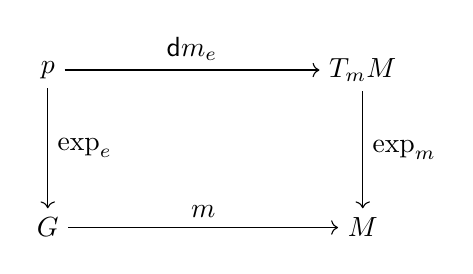
\begin{tikzpicture}
\node (PF) at (0,2) [] {$\pf$};
\node (TM) at (4,2) [] {$T_mM$};
\node (M) at (4,0) [] {$M$};
\node (G) at (0,0) [] {$G$};

\draw [->] (PF) -> (TM) node[midway, above] {$\d \m_e$};
\draw [->] (TM) -> (M) node[midway, right] {$\exp_m$};
\draw [->] (G) -> (M) node[midway, above] {$\m$};
\draw [->] (PF) -> (G) node[midway, right] {$\exp_e$};
\end{tikzpicture}
\end{center}
\begin{Beweis}{}
Setze $c(t) := c_{\d \m_eX}(t)$. Dann gilt
\[ c(t) = \tau_t.c(0) = \tau_t.m \]
für $\tau_t = s_{c(t/2)}\circ s_m$. Es folgt
\[ \tau_t = \exp(tZ) \]
für ein $Z \in \g$. Die Behauptung $Z = X$ folgt, wenn wir zeigen können, dass
\[ Z \in \pf \]
da $\m(\tau_t) = c(t)$. Nun gilt tatsächlich
\[ \sigma(\tau_t) = s_m s_{c(t/2)} s_m s_m = s_m \circ s_{c(t/2)} = s_{c(-t/2)}\circ s_m = \tau_{-t} \]
ergo
\[ \d \sigma_e(Z) = -Z \]
ergo $Z \in \pf$.
\end{Beweis}

\Def{}
Ein glattes Vektorfeld $V \in \V(M)$ heißt \df{Killing-Feld}, falls für alle Vektorfelder $Y,Z$ gilt
\[ \L_X g(Y,Z) = g(\D_X Y, Z) + g(Y, \D_X Z) = 0 \]
$\L_X$ bezeichnet hier die \df{Lie-Ableitung}.\\
Unter $\g^*$ verstehen wir die Lie-Algebra der Killing-Felder auf $M$. Ein Killing-Feld $X^*$ ist festgelegt durch $X^*(m)$ und die Abbildung $\D X^*(m)$.\\
Setze
\begin{align*}
\kf^* &= \{X^* \in \g^*~|~X^*(m) = 0\}\\
\pf^* &= \{X^* \in \g^*~|~\D X^*(m) = 0\}
\end{align*}

\Bem{}
Betrachte
\begin{align*}
\pf^* & \Pfeil{} T_mM\\
X^* & \longmapsto X^*(m)
\end{align*}
und
\[ \kf = \set{A \in End(T_mM) = O(T_mM, g_m)}{ \forall u,v \in T_mM: A \circ \Rc_m(u,v) = \Rc_m(Au,v) + \Rc_m(u,Av) + \Rc(u,v) \circ A } \]
wobei $g_m$ die Metrik bei $m$ und $\Rc$ den Krümmungstensor bei $m$ bezeichnet.\\
Auf $End(T_mM)$ ergibt sich eine Lie-Algebren-Struktur durch
\[ [A,B] := A\circ B - B\circ A \]
Die Abbildung
\begin{align*}
\Phi: \kf^* & \Pfeil{} \kf\\
X^* & \longmapsto \D X^*(m)
\end{align*}
ist ein Anti-Isomorphismus von Lie-Algebren, d.\,h., ein Isomorphismus von Vektorräumen, für den gilt
\[ \D [X^*,Y^*](m) = \Phi([X^*, Y^*]) = [\Phi(Y^*), \Phi(X^*)] = [\D_{Y^*}, \D_{X^*}](m) \]
Ferner ist
\[ \D_{U,X^*}^2Y^* := \D_U \D_{X^*}Y^* - \D_{\D_UX^*}Y^* \]
tensoriell in $X^*,Y^*$ und es gilt
\[ \D_{U,X^*}^2Y^* = - \Rc(X^*, U)Y^* \]

\Prop{}
Es gilt
\begin{enumerate}[1.)]
\item $[\kf^*, \kf^*] \subset \kf^*, [\kf^*, \pf^*] \subset \pf^*$ und $[\pf^*, \pf^*] \subset \kf^*$
\item Für alle $X^*,Y^* \in \pf^*$ gilt
\[ \D [X^*, Y^*](m) = \Rc_m(X^*(m),Y^*(m)) \]
\item Für alle $X^*\in \kf^*, Y^* \in \pf^*$ gilt
\[ [ Y^*, X^* ](m) = \D_{Y^*(m)}X^*(m)  \]
und
\[ \D_{X^*(m)}Y^*(m) = 0 \]
\end{enumerate}
\begin{Beweis}{}
\begin{enumerate}[1.)]
\item \[  \D_{Y^*(m)}X^*(m) = \D_{Y^*(m)}X^*(m) - \D_{X^*(m)}Y^*(m) = [ Y^*, X^* ](m)   \]
\item 
\begin{align*}
\D_W[X^*,Y^*](m) &= \D_W(\D_{X^*}Y^* - \D_{Y^*}X^*)\\
 &= \D_W\D_{X^*}Y^* - \D_W\D_{Y^*}X^*\\
 &\gl{ \D_WX^* = 0 } \D_W\D_{X^*}Y^* - \D_{\D_WX^*}Y^*- \D_W\D_{Y^*}X^* + \D_{\D_WY^*}X^*\\
 &= \D_{W,X^*}^2Y^* - \D_{W,Y^*}^2X^*\\
 &= - \Rc(Y^*,W)X^* + \Rc (X^*,W)Y^*\\
 &\gl{1.Bianchi} \Rc(X^*,Y^*)W
\end{align*}
\end{enumerate}

\end{Beweis}

\Kor{}
\[ \Rc_m(X^*,Y^*)W^* = [W^*,[X^*,Y^*]](m) \]

\Bem{}
$\kf$ ist die Lie-Algebra der kompakten Gruppe $K$. Betrachte die Killing-Form auf $\kf$
\[ B_{\kf} (A,B) = spur(ad(A) \circ ad(B)) \]
diese ist negativ definit und $ad(\kf)$-invariant. Bezeichnet $\shrp{,}_M$ das Skalarprodukt auf $\pf \isom{} T_mM$, so erhalten wir auf $\g$ durch
\[ \shrp{,} := \shrp{,}_M - B_\kf \]
ein Skalarprodukt, welches $ad(\kf)$- und $\d \sigma_e$-invariant ist.

\Def{}
Eine \df{orthonormale involutive Lie-Algebra} $\g$ besteht aus einer Involution $\sigma$ und einem Skalarprodukt, welches $\sigma$- und $ad(\kf)$-invariant ist, wobei $\kf$ den 1-Eigenraum von $\sigma$ bezeichnet.

\Def{}
Sei $\g$ eine orthonormale involutive Lie-Algebra, dann ist $\shrp{,}_{|\pf}$ positiv definit und es existiert eine Konstante $\lambda$, sodass für die Killing-Form gilt
\[ B_{|\pf} = \lambda \cdot \shrp{,}_{|\pf} \]
\begin{itemize}
\item $\g$ heißt \df{euklidisch}, falls $\lambda = 0$
\item $\g$ heißt \df{von nicht-kompakten Typ}, falls $\lambda > 0$
\item $\g$ heißt \df{von kompakten Typ}, falls $\lambda < 0$
\end{itemize}

\Bsp{}
\begin{enumerate}[1.)]
\item $(o(n), \sigma, \shrp{,})$ ist von kompakten Typ, $K = O(p)\times O(q)$
\item $(o(p,q), \sigma_1, \shrp{,})$ ist von nicht-kompakten Typ, $K = O(p)\times O(q)$
\item $(\slf, \sigma, \shrp{,})$ ist von nicht-kompakten Typ, $K = \SO$
\end{enumerate}

\Satz{Dualität}
Sei $\g = \kf \oplus \pf$ eine orthonormale involutive Lie-Algebra, dann ist
\[ \g_* = \kf \oplus i \cdot \pf \]
eine orthonormale involutive $\C$-Sub-Lie-Algebra von $\g \otimes \C$. Es gilt dann
\begin{itemize}
\item $\g$ ist genau dann von kompakten Typ, wenn $\g_*$ von nicht-kompakten Typ ist.
\item $\g$ ist genau dann von nicht-kompakten Typ, wenn $\g_*$ von kompakten Typ ist.
\end{itemize}

\Bem{Schnittkrümmung}
Seien $u,v \in T_mM$ normiert und orthogonal. Dann gilt
\begin{align*}
\kappa(u,v) &= g(\Rc(u,v)v, u)\\
&= \lambda\i B_{|\pf}(\Rc(u,v)v,u)\\
&= \lambda\i B([v,[u,v]],u)\\
&= \lambda\i B([u,v],[v,u])\\
&= -\lambda\i B([u,v],[u,v])\\
\end{align*}
Ist $\g$ also von kompakten Typ, so ist $M$ nicht-negativ gekrümmt. Ist $\g$ von nicht-kompakten Typ, so ist $M$ nicht-positiv gekrümmt.\\
Gilt in einem der Fälle
\[ [u,v] = 0 \]
so folgt dann
\[ \kappa(u,v) = 0 \]

\Bsp{}
\begin{enumerate}[1.)]
\item Betrachte
\[ \of(n) = \set{A\in\R^{n\times n}}{-A = A^T} \]
mit
\[ B(X,Y) = spur(ad(X) \circ ad(Y)) = \lambda \cdot spur(X\cdot Y) \]
für $\lambda > 0$ konstant, und
\[ ad(X)A = [X,A] = XA -AX \]
Dann gilt
\[ B(X,X) = \lambda spur(XX) = \lambda spur(-X^TX) = -\lambda \sum_{i=1}^n x_i^2 < 0 \]
wenn nicht alle Eigenwerte $x_i$ von $X$ verschwinden. D.\,h., $B_{|\pf}$ ist von negativem Typ, ergo ist $\of(n)$ von kompakten Typ.
\item Betrachte $\slf$ mit $\pf = \symm$, dann gilt
\[ B_{|\pf} = spur(XX) = spur(X^TX) = \sum_{i =1}^nx_i^2 > 0 \]
ergo ist $\slf$ von nicht-kompakten Typ.
\end{enumerate}

\printindex
\end{document}